\documentclass[%
reprint,
superscriptaddress,
%groupedaddress,
%unsortedaddress,
%runinaddress,
%frontmatterverbose,
%preprint,
showpacs,preprintnumbers,
%nofootinbib,
%nobibnotes,
%bibnotes,
amsmath,amssymb,
aps,
%pra,
%prb,
prd,
%prl,
%rmp,
%prstab,
%prstper,
%floatfix,
]{revtex4-1}

\usepackage{float}
\usepackage{graphicx}% Include figure files
\usepackage{dcolumn}% Align table columns on decimal point
\usepackage{bm}% bold math
\usepackage{bbold}
\usepackage{braket}
\usepackage{amssymb,amsmath}
\usepackage{hyperref}% add hypertext capabilities
%\usepackage[mathlines]{lineno}% Enable numbering of text and display math
%\linenumbers\relax % Commence numbering lines

%\usepackage[showframe,%Uncomment any one of the following lines to test
%%scale=0.7, marginratio={1:1, 2:3}, ignoreall,% default settings
%%text={7in,10in},centering,
%%margin=1.5in,
%%total={6.5in,8.75in}, top=1.2in, left=0.9in, includefoot,
%%height=10in,a5paper,hmargin={3cm,0.8in},
%]{geometry}



\usepackage{color}
\usepackage[dvipsnames, svgnames, x11names]{xcolor}
\usepackage{amsfonts}
\usepackage{subfigure}
\usepackage{array}


\newcommand{\Tr}{\ensuremath{\operatorname{Tr}}}
\newcommand{\tr}{\ensuremath{\operatorname{tr}}}
\newcommand{\Omegaqq}{\ensuremath{\Omega_{\bar{q}q}}}
\newcommand{\vev}[1]{\ensuremath{\left\langle #1 \right\rangle}}
\newcommand{\einh}[1]{\ensuremath{\,\text{#1}}}
\newcolumntype{L}{>{\centering\arraybackslash}m{3cm}}



\newcommand{\overbar}[1]{\mkern 1.5mu\overline{\mkern-1.5mu#1\mkern-1.5mu}\mkern 1.5mu}

\definecolor{bjcol}{rgb}{1,.44,0.13}

% color def's

\definecolor{blue}{rgb}{0,0,1}
\newcommand{\colb}[1]{{\color{blue} #1}}
\definecolor{green}{rgb}{0,1,0}
\newcommand{\colg}[1]{{\color{green} #1}}
\definecolor{red}{rgb}{1,0,0}
\newcommand{\colr}[1]{{\color{red} #1}}
\newcommand{\colJ}[1]{{\color{cyan} #1}}
\definecolor{gray}{rgb}{.5,.5,.5}
\newcommand{\drop}[1]{{\sout{ {\color{gray} #1}}}}
\definecolor{darkgreen}{rgb}{.0,.5,.0}
\newcommand{\colL}[1]{{\color{darkgreen} #1}}


\def\Fig#1{Fig.~\ref{#1}} \def\Tab#1{Tab.~\ref{#1}}
\def\Figs#1{Figs.~\ref{#1}} \def\Tab#1{Tab.~\ref{#1}}
\def\Eqs#1{Eqs.~(\ref{#1})}
\def\Eq#1{Eq.~(\ref{#1})}
\def\eq#1{(\ref{#1})}
\def\eqref#1{(\ref{#1})}
\def\fig#1{Fig.~\ref{#1}}
\def\tab#1{Tab.~\ref{#1}}
\def\eqs#1{(\ref{#1})}
\def\Eqs#1{(\ref{#1})}
\def\sec#1{Sec.~\ref{#1}}
\def\app#1{Appendix~\ref{#1}}
\newcommand{\Phibar}{\ensuremath{\bar{\Phi}}}
\newcommand{\LPQM}{\ensuremath{\mathcal{L}_{\textrm{PQM}}}\xspace}

\def\dbar{{\mathchar'26\mkern-12mu d}}
\def\lA0{{\langle A_0 \rangle}}
\def\bA0{{\bar{A}_0}}
\def\lLA{{\langle L[A_0] \rangle}}
\def\lL{{\langle L \rangle}}
\def\lLc{{\langle L^\dagger \rangle}}
\def\lLAc{{\langle L^\dagger[A_0] \rangle}}


\def\dr{{D\!\llap{/}}\,}
\def\Dr{{D\!\llap{/}}\,}
\def\ipv{\vec{p}\llap{/}}
\def\pslash{p\llap{/}}

\def\0#1#2{\frac{#1}{#2}}

\newcommand{\bsig}{\ensuremath{\bar{\sigma}}}
\newcommand{\lsm}{L\ensuremath{\sigma}M\xspace}
\newcommand{\pT}{\ensuremath{T_0}}
\newcommand{\Tl}{\ensuremath{T_\chi}}
\newcommand{\Ts}{\ensuremath{T_\chi^s}}
\newcommand{\Tchi}{\ensuremath{T_\chi}}
\newcommand{\Td}{\ensuremath{T_d}}
\newcommand{\Tc}{\ensuremath{T_c}}
\newcommand{\muc}{\ensuremath{\mu_c}}
\newcommand{\coloronl}{(color online)\xspace}

\newcommand{\mrm}[1]{\mathrm{#1}}
\def\qbar{\bar{q}}
\newcommand{\sx}{\sigma_{x}}
\newcommand{\sy}{\sigma_{y}}

%%%%%%%%%%%%% Hypersetup %%%%%%%%%%%%%

\newcommand{\gettitle}{Chiral and effective $U(1)_{\rm A}$ symmetry restoration in QCD}

\renewcommand{\figureautorefname}{Fig.}
\renewcommand{\sectionautorefname}{Sec.}
\renewcommand{\subsectionautorefname}{Subsec.}
%\renewcommand{\appendixautorefname}{App.}
\def\appendixautorefname{App.}

%\hypersetup{
%	colorlinks,
%	linkcolor={blue!75!black},
%	citecolor={blue!75!black},
%	urlcolor={blue!75!black},
%	%%%%%%%%%%%%%%%%%%%%%%%%%%%%%%%%%%
%	pdftitle={\gettitle},
%	pdfauthor={},
%	pdfkeywords={Renormalization group} {HIC}
%	{Correlations functions} {hyperfluctuations},
%	bookmarksopen=true,
%	bookmarksopenlevel=2,
%	bookmarksnumbered=true
%}


%%%%%%%%%%%%%% for corrections %%%%%%%%%%%
\newcommand{\colwj}[1]{\textcolor{Purple}{#1}}
\newcommand{\colxf}[1]{\textcolor{cyan}{#1}}
\newcommand{\coljan}[1]{\textcolor{red}{#1}}
\newcommand{\colfab}[1]{\textcolor{magenta}{#1}}
\newcommand{\colrui}[1]{\textcolor{green}{#1}}
\newcommand{\colnu}[1]{\textcolor{blue}{#1}}
\newcommand{\colshi}[1]{\textcolor{Plum}{#1}}

%
%%%%%%%%%%%%%%%%%%%%%%%%%%%%%%%%%%%%%%%%%%%%%%%%%%%%%%%%%%%%%%%%%%%%%%%%%%%%%

\graphicspath{{./figures/}{./}}

\begin{document}
	
	\preprint{}
	
	\title{Hyper-order baryon number fluctuations at finite temperature and density}
	
	
	
	\affiliation{Key Laboratory of Quark \& Lepton Physics (MOE) and Institute of Particle Physics,
		Central China Normal University, Wuhan 430079, China}
	
	\author{Wei-jie Fu}
	\affiliation{School of Physics, Dalian University of Technology, Dalian, 116024,
		P.R. China}
	
	\author{Xiaofeng Luo}
	\affiliation{Key Laboratory of Quark \& Lepton Physics (MOE) and Institute of Particle Physics,
		Central China Normal University, Wuhan 430079, China}
	
	\author{Jan M. Pawlowski}
	\affiliation{Institut f\"ur Theoretische Physik, Universit\"at Heidelberg, Philosophenweg 16, 69120 Heidelberg, Germany}
	\affiliation{ExtreMe Matter Institute EMMI, GSI, Planckstra{\ss}e 1, D-64291 Darmstadt, Germany}
	
	\author{Fabian Rennecke}
	\affiliation{Physics Department, Brookhaven National Laboratory, Upton, NY 11973, USA}
	
	\author{Rui Wen}
	\affiliation{School of Physics, Dalian University of Technology, Dalian, 116024,
		P.R. China}
	
	\author{Shi Yin}
	\affiliation{School of Physics, Dalian University of Technology, Dalian, 116024,
		P.R. China}
	
	
	%\date{\today}% It is always \today, today,
	%  but any date may be explicitly specified
	
	\begin{abstract}
		
		We study the fourth- to tenth order (hyper-order) baryon number fluctuations at finite temperature and density in a  QCD-assisted low energy effective theory that includes low energy quantum, thermal and density fluctuations. At vanishing density our results agree quantitatively, both with lattice QCD simulations for temperatures $T\gtrsim 140$\, MeV, and with the hadron resonance gas for $T\lesssim 120$\,MeV. We then compute baryon number fluctuations at different collision energies, which is compared with recent experimental measurements of the kurtosis and the sixth-order cumulant of the net-proton distribution from the STAR collaboration. 
		
		The current approach shows a non-monotonic behavior of higher order cumulants as a function of the beam-energy measured by STAR, even though the QCD-assisted low energy effective theory used shows no critical behaviour in the respective regime. This asks for a refined analysis and interpretation of hyper fluctuations within first principles QCD, whose setup is also discussed here.  
		
	\end{abstract}
	%\pacs{Valid PACS appear here}% PACS, the Physics and Astronomy
	\pacs{11.30.Rd, %Chiral symmetries
		11.10.Wx, %Finite-temperature field theory
		05.10.Cc, %Renormalization group methods
		12.38.Mh  %Quark-gluon plasma
	}                             % Classification Scheme.
	%\keywords{Suggested keywords}%Use showkeys class option if keyword
	%display desired
	\maketitle
	%\tableofcontents
	
	%%%%%%%%%%%%%%%%%%%%%%%%%%%%%%%%%%%%%%%%%%%%%%%%%%%%%%%%%%%
	%%%%%%%%%%%%%%%%%%%%%%%%%%%%%%%%%%%%%%%%%%%%%%%%%%%%%%%%%%%
	
	\section{Introduction}
	\label{sec:int}
	
	One of the most intriguing open questions concerning the QCD phase diagram is the potential existence of a seoncd order critical end point (CEP) at higher densities. Unravelling existence of the  CEP, as well as its location and critical dynamics, plays a pivotal role in understanding phases of strongly interacting nuclear matter under extreme conditions. For works on the phase structure of QCD, covering Experiment and Theory see  \cite{Stephanov:2007fk, Luo:2017faz,Bzdak:2019pkr,Fischer:2018sdj,Fu:2019hdw} \coljan{Lattice, CBM/NICA is missing}, where theory covers first principles functional approaches and lattice simulations.
	
	Critical observables, such as fluctuations of conserved charges diverge due to the critical dynamics in the proximity of the CEP \cite{Stephanov:2008qz}. Accordingly, these are natural observables for locating the CEP  as well as revealing its dynamics \cite{Luo:2017faz,Adam:2020unf}. It has been proposed in \cite{Stephanov:1999zu, Stephanov:2008qz, Stephanov:2011pb}, that non-monotonic variations of conserved charge fluctuations as functions of the beam energy could signal the presence of a CEP. 
	
	Within the Beam Energy Scan (BES) Program at the Relativistic Heavy Ion Collider (RHIC), significant fluctuation measurements have been performed in Phase I, involving the skewness and kurtosis of the net-proton, net-charge, net-kaon multiplicity distributions  \cite{Adamczyk:2013dal,Adamczyk:2014fia,Luo:2015ewa,Adamczyk:2017wsl}, second-order off-diagonal cumulants, i.e., correlations of net-proton, net-charge, net-kaon multiplicity distributions \cite{Adam:2019xmk}. Remarkably, very recently the STAR collaboration has reported the first evidence of a non-monotonic variation in kurtosis $\times$ variance of the net-proton number distribution as a function of the collision energy with $3.0\sigma$ significance for central collisions \cite{Adam:2020unf}. The measurements have been extended to the sixth-order cumulant of net-proton and net-charge distributions, for preliminary results see  \cite{Nonaka:2020crv,Pandav:2020uzx}.
	
	Remarkably, recent first-principle QCD calculations at finite temperature and density, within both the functional renormalization group (fRG) and Dyson-Schwinger equations (DSE), indicate that the location of CEP is presumably in a region of $450\,\mathrm{MeV} \lesssim\mu_B\lesssim 650\,\mathrm{MeV}$ \cite{Fischer:2018sdj,Fu:2019hdw,Isserstedt:2019pgx,Gao:2020qsj, Gao:2020fbl}. This entails, that one has to explore the high-$\mu_B$ region with $\mu_B/T_c\gtrsim 4$. 
	
	In this regime fluctuations and correlations of conserved charges, e.g., has been intensively studied within functional approaches. In the present work, we build upon previous investigations  of the skewness and kurtosis of baryon number distributions \cite{Fu:2015naa,Fu:2015amv,Fu:2016tey}, and baryon-strangeness correlations \cite{Fu:2018qsk,Fu:2018swz} within QCD-assisted low energy effective theories (LEFT) with the fRG. For further  investigations within the functional renormalisation group approach to low energy effective theories see e.g.\  \cite{Skokov:2010wb,Skokov:2010uh,Morita:2014fda,Almasi:2017bhq}, the Dyson-Schwinger approach has been used in e.g.\  \cite{Xin:2014ela,Isserstedt:2019pgx}, for mean-field investigations see e.g.\ \cite{Fu:2009wy,Fu:2010ay,Karsch:2010hm,Schaefer:2011ex,Li:2018ygx}. These functional works can be adjusted and benchmarked with results from lattice QCD simulations  \cite{Bazavov:2012vg,Borsanyi:2013hza,Borsanyi:2014ewa,Bazavov:2017dus,Bazavov:2017tot,Borsanyi:2018grb,Bazavov:2020bjn}, at high temperatures, $T\gtrsim T_c$, and vanishing $\mu_B$. In turn, at finite-$\mu_B$, and in particular for $\mu_B/T_C\gtrsim 3$, lattice simulations are obstructed by the sign problem. 
	
	Apart from systematically improving the approach and results within the QCD-assisted LEFT approach in  \cite{Fu:2015naa,Fu:2015amv,Fu:2016tey}, we also provide results for  hyper-order baryon number fluctuations (orders higher than four). The reliability of the results for these fluctuations is qualitatively improved by utilising imput from QCD (hence  'QCD-assisted') and heavy-ion phenomenology. This includes scale-matching relations benchmarked and tested in two- and 2+1 flavour QCD with results from \cite{Fu:2019hdw} . 
	
	
	More specifically, we use first-principles QCD results on the $T$-dependence of the kurtosis and the $\mu_B$-dependence of the chiral phase boundary to map the in-medium scales of the LEFT onto QCD. This will improve the reliability of our predictions for the hyper-order fluctuations. Furthermore, phenomenological freeze-out curves will be used to map our results in terms of $T$ and $\mu_B$ onto the beam energies of heavy-ion collisions.
	This allows us to compare our calculations with recent results of lattice simulations in the regime of low $\mu_B$ and experimental data in \cite{Adam:2020unf,Nonaka:2020crv,Pandav:2020uzx}, but also to make predictions for hyper-order fluctuations. Implications of the comparison will be discussed in detail.
	
	The present QCD-assisted LEFT approach has various advantages. Most importantly, it is directly embedded in QCD as the relevant low-energy degrees of freedom emerge dynamically from systematically integrating-out the fast partonic modes of QCD \cite{Mitter:2014wpa, Braun:2014ata, Rennecke:2015eba, Cyrol:2017ewj, Fu:2019hdw}. In addition, such an approach allows us to capture both critical and non-critical effects in the QCD phase diagram. In particular we can disentangle clear \textit{signatures} of the critical region close to a CEP from \textit{indications} for a CEP: 
	
	The former \textit{signatures} or smoking gun is given by critical scaling and divergences in the (hyper-order) fluctuations. In turn, the latter \textit{indications} is provided with the non-monotonous behaviour of the fluctuations: they necessarily arise in the critical region, but are known to be also present far away from it. The occurence of the latter in the QCD-assisted LEFT used here offers compelling evidences for this, and is discussed in detail. In conclusion this clear distinction is indispensable for the accurate interpretation of the experimental results, especially since there is also evidence that critical physics can only be observed in a very small region around the CEP, see e.g.\ \cite{Schaefer:2006ds}. 
	
	This paper is organized as follows: In \autoref{sec:FRG} we give a brief introduction about the fRG flows of QCD and low energy effective theory and their mutual relationship. Thermodynamics and the hyper-order baryon number fluctuations are discussed in \autoref{sec:hyper-fluc}. In \autoref{sec:num}, first of all, we match the scale between QCD and the low energy effective theory, and then, the calculated results are compared with the lattice QCD simulations and experimental measurements. A summary with conclusions is given in \autoref{sec:summary}. Moreover, details of glue potential and flow equations are presented in \hyperref[app:gluepot]{App.~\ref{app:gluepot}} and \hyperref[app:flowV]{App.~\ref{app:flowV}}, respectively.
	
	
	
	
	%%%%%%%%%%%%%%%%%%%%%%%%%%%%%%%%%%%%%%%%%%%%%%%%%%%%%%%%%%%%%
	%%%%%%%%%%%%%%%%%%%%%%%%%%%%%%%%%%%%%%%%%%%%%%%%%%%%%%%%%%%%%
	
	\section{QCD and emergent low energy effective theories}
	\label{sec:FRG}
	
	%
	%%%%%%%%%%%%%%%%%%%%%%%%%%%%
	\begin{figure}[t]
		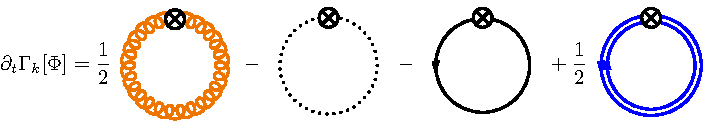
\includegraphics[width=0.45\textwidth]{QCD_equation}
		\caption{Diagrammatic representation of the QCD flow equation within the fRG approach. Lines of different types on the r.h.s. of the equation stand for the full propagators of gluon, ghost, quark, and meson, respectively. Note that the mesonic degree of freedom is denoted by double lines with opposite arrows. The crossed circles represent the regulators in the flow equation.}\label{fig:QCD_equation}
	\end{figure}
	%%%%%%%%%%%%%%%%%%%%%%%%%%%%%
	%
	
	At low momentum scales the glue-dynamics of QCD successively decouples due to the QCD mass gap. This decoupling also applied to the dynamical (hadronic) low energy degrees of freedom, finally leaving us with dynamical pions and hence with chiral perturbation theory ($\chi$PT). Indeed, this successive decpoupling is at the root of the success of $\chi$PT. 
	
	The functional renormalisation group approach to QCD with its successive integrating-out of momentum modes is ideally suited to follow and study this decoupling. Diagrammatically, this is already seen within the flow equation for the QCD effective action, depicted in \autoref{fig:QCD_equation}. The different lines stand for the full non-perturbative propagators of gluon, ghost, quark and for effective hadronic low energy degrees of freedom and the loop momentum $q$ is restricted by the infrared cutoff scale $k$, $q^2\lesssim k^2$. The latter emerged within dynamical hadronisation in QCD and do not signal a low energey effective theory, \cite{Gies:2001nw, Gies:2002hq, Pawlowski:2005xe, Floerchinger:2009uf}. For quantitative QCD applications in the vacuum see \cite{Braun:2014ata, Rennecke:2015eba, Mitter:2014wpa, Cyrol:2017ewj} in the vacuum, for further conceptual developments and the application to the QCD phase structure important for the present work see \cite{Fu:2019hdw}. The decoupling is now very apparent as the propagators carry the mass gaps $m_\textrm{gap}$ of quarks, gluons and quarks and for cutoff scales $k\ll m_\textrm{gap}$ of a given field the respective loop tends towards zero. 
	
	More importantly, in this way the emergent low energy effective theory is naturally embedded in QCD, and its ultraviolet parameters (at $\Lambda\lesssim1$\,GeV) as well as further input may be directly computed from QCD, leading to \textit{QCD-assisted} low energy effective theories. For more details see in particular \cite{Fu:2019hdw}, and the recent review \cite{Dupuis:2020fhh}. Most prominently this embedding has been used for determining the temperature-dependence of the Polyakov loop potential, see \cite{Haas:2013qwp, Herbst:2013ufa}. This setup was then applied to the computation of fluctuations in \cite{Fu:2015amv, Fu:2015naa, Fu:2016tey,Wen:2018nkn,Yin:2019ebz}. 
	
	
	In summary this entails, that for sufficiently small momenta $k2$, temperatures $T$, and also density or quark chemical potential $\mu_q$, the gluon (and ghost) loop in \autoref{fig:QCD_equation} decouple from the dynamics, and only provide a non-trivial glue background at finite temperature and chemical potential. The latter is taken into account with the Polyakov loop potential discussed in detail later. 
	
	\subsection{Two-flavour setup}\label{sec:Nf2LEFT}
	For the physics of fluctuations we are interested in $k,T, \mu_B\lesssim 1$\,GeV. We restrict ourselves to $k\lesssim 700$\,MeV and temperatures and quark chemical potentials $T,\mu_q \lesssim 200$\,MeV. In this regime we are left with the light quarks $q=(u,d)$ and the strange quark $s$. The latter, while changing the momentum-scale running of the correlation functions, has subleading effects on the form of the fluctuations. Hence, the effect of the momentum-scale running induced by strange fluctuations, will be mimic here by an appropriate scale matching detailed in \autoref{subsec:scale}. We also the lowest lying hadronic resonances, the pion ${\bm\pi}=(\pi^\pm,\pi^0)$, and for symmetry reasons, the scalar resonance $\sigma$. The other members of the lowest lying multiplet as well as further hadronic resonances produce rather subleading contributions to the offshell dynamics and hence are dropped. The mesonic fields are stored in an O(4) scalar field $\phi=(\sigma, {\bm\pi})$. Quantum, thermal and density fluctuations with scales $k\lesssim \Lambda= 700$\,MeV are taken into account within the fRG, whose dynamics is now reduced to the last two loops in \autoref{fig:QCD_equation}. The respective effective action of QCD in the low energy regime is approximated by 
	%The direct consequence of the natural emergence of LEFT is that,  if the flow equation of QCD in \Eq{eq:QCDflow} is evolved from an initial scale where the glue sector has already been suppressed significantly by the gluon mass gap, \colfab{say $\Lambda < 1$ GeV}, it is safe and legitimate to disregard quantum fluctuations of the glue sector, i.e., the first two diagrams in \Fig{fig:QCD_equation}. Hence we are left with a scale dependent effective action in Euclidean spacetime, only composed of the dynamical matter fields, namely quarks and mesons, which reads
	%
	\begin{align}
		\Gamma_k=&\int_x \bigg\{Z_{q,k}\bar{q} \Big [\gamma_\mu \partial_\mu -\gamma_0(\hat\mu+igA_0) \Big ]q+\frac{1}{2}Z_{\phi,k}(\partial_\mu \phi)^2 \nonumber\\[2ex]
		&\hspace{.3cm}+h_k\,\bar{q}\,
		\left(\tau^0\sigma+\bm\tau
		\cdot\bm{\pi}\right)\,q +V_k(\rho,A_0)-c\sigma \bigg\}\,,\label{eq:action}
	\end{align}
	%
	with $\int_{x}=\int_0^{1/T}d x_0 \int d^3 x$ and
	$\tau=1/2 (\mathbb{1}, i \gamma_5 \bm \sigma)$. In \eq{eq:action}, 
	%a reduction of the involved species of fields $\Phi=(q,\bar q,\phi)$, and 
	%i.e., the quark field $q=(u\,,d)^{T}$ in the action \Eq{eq:action}. The meson field $\phi=\left(\sigma,\vec{\pi}\right)$, being in the adjoint representation of group $\mathrm{U_V}(N_f)\times\mathrm{U_A}(N_f)$ in the flavor space, is coupled with the quark field through the Yukawa coupling. Here $T^0$ and $T^{i}$'s ($i=1\,,2\,,\cdots\,,N_f^2-1$) are the generators of $\mathrm{U}(N_f)$ group, denoted collectively as $T^a$'s, with the normalization $\Tr(T^{a}T^{b})=\frac{1}{2}\delta^{ab}$, which yields $T^{0}=\frac{1}{\sqrt{2N_{f}}}\mathbb{1}_{N_{f}\times N_{f}}$. 
	$Z_{q,k}$ and $Z_{\phi,k}$ are the wave function renormalisations for the light quarks and the meson respectively. Further running couplings considered are the Yukawa coupling $h_k$, the scattering between quarks and mesons, as well as the effective potential $V_k(\rho,A_0)$, that describes the multi-scattering of mesons in the non-trivial glue background present at finite temperature and chemical potential.
	
	The flow equation for the effective action \eq{eq:action}, and that for $V_k, h_k, Z_{\phi,q}$ is described in \autoref{app:fRG} and \autoref{app:flowV}. The initial condition for $\Gamma_k$ at the initial cutoff scale $k=700$\,MeV is described in \autoref{app:Ini}. 
	
	The potential $V_k(\rho, A_0)$ has contributions $V_{\mathrm{glue},k}(A_0)$ from offshell glue fluctuations (first two diagrams in \autoref{fig:QCD_equation}), and contributions $V_{\mathrm{mat},k}(\rho,A_0)$ from the quark loop (third diagram in \autoref{fig:QCD_equation}). This leads us to 
	%
	\begin{align}
		V_k(\rho,A_0)=&V_{\mathrm{glue},k}(A_0)+V_{\mathrm{mat},k}(\rho,A_0)\,,\label{eq:Vtotal}
	\end{align}
	%
	The first contribution is typically reformulated in terms of the Polyakov loop $L(A_0)$, while the latter is directly computed from the present low energy flow. This allows us to trade the $A_0$-dependence for that of the traced Polyakov loop, $L(A_0), \bar L(A_0)$, see \autoref{app:gluepot}, \eq{eq:Lloop}, leading us to to the final form of our potential, 
	%
	\begin{align}
		V_k(\rho, L,\bar L)= V_k(\rho, A_0)\,. 
	\end{align}
	More details about $V_{\mathrm{glue},k}$ used in this work can be found in \autoref{app:gluepot}. 
	
	\subsection{$2+1$-favour scale matching in $2$-flavour QCD}
	\label{subsec:scale}
	
	The current QCD-assisted LEFT setup enables us to compute thermodynamic observables and in particular hyper-order baryon number fluctuations. However, as already briefly discussed in \autoref{sec:Nf2LEFT}, we have dropped the dynamics of the strange quark. While we expect sub-dominant effects on hyper-fluctuations, the $s$-quark influences the momentum running of the correlations in the ultraviolet. 
	
	Importantly, in \cite{Fu:2019hdw} it has been observed on the basis of genuine $N_f=2$ and $N_f=2+1$ flavour computations in QCD, that the latter effect is well approximated by a respective universal scale-matching of the two-flavour results even in QCD. Such a scale-matching has already led to a rather quantitative agreement of thermodyanmics and kurtosis within the current LEFT setup with lattice results, see \cite{Fu:2015amv, Fu:2015naa, Fu:2016tey}. 
	
	
	Given its relevance for the predictive power of the present LEFT within a QCD scale matching we briefly recall the respective results in \cite{Fu:2019hdw}: There, the phase boundary of two- and $2+1$-flavour QCD has been computed within the fRG approach. The results there allows us to evaluate the reliability of even linear scale-matchings of temperatures and chemical potentials in two- and 2+1-flavour QCD introduced by 
	%
	\begin{align}
		T^{(N_f=2)} &=c_{_{T}}\,T^{(N_f=2+1)} \,, \quad \mu_B^{(N_f=2)} =c_{\mu_B}\,\mu_{B}^{(N_f=2+1)} \,,\label{eq:rescale}
	\end{align}
	%
	With such a linear scale-matching the scaling factors $c_{_{T}}, c_{\mu_B}$ can be determined by evaluating the relations at a specific temperature and chemical potential. Naturally we take $(T,\mu_B)=(T_c,0)$, the crossover temperature at vanishing chemical potential. 
	
	In \cite{Fu:2019hdw} the crossover temperatures have been determined with thermal susceptibilities of the renormalised light chiral condensate. Then, the linear rescaling of the two-favour chiral crossover temperature to the 2+1-flavour crossover temperature is done with 
	%
	\begin{align}\label{eq:cTQCD}
		T_c^{(N_f=2)} = c_T^{\textrm{QCD}}\, T_c^{(N_f=2+1)}\,, \qquad  c_T^{\textrm{QCD}}=1.1\,. 
	\end{align} 
	For the matching of the chemical potentials we use the curvature $\kappa$ of the phase boundary at vanishing $\mu_B=0$, 
	%
	\begin{align}
		\frac{T_c(\mu_B)}{T_c}&=1-\kappa \left(\frac{\mu_B}{T_c}\right)^2+\lambda \left(\frac{\mu_B}{T_c}\right)^4+\cdots\,.\label{eq:curv}
	\end{align}
	% 
	\Eq{eq:curv} already entails that the curvature is invariant if the chemical potential and temperature are rescaled with the same value, and thus the curvature $\kappa_{_{LEFT}}$ in the LEFT would not be modified if one has $c_{\mu}=c_{_{T}}$ in \Eq{eq:rescale}. 
	
	Adjusting the two-flavour curvature $-\kappa \mu_B^2/T_c^2$ to the 2+1-flavour one leads us to the relation 
	%
	\begin{align}
		c^\textrm{QCD}_{\mu}&=c^{\textrm{QCD}}_{_{T}}\left(\frac{\kappa^{(N_f=2+1)}}{\kappa^{(N_f=2)}}\right)^{1/2}\,, \qquad c_{\mu}^\textrm{QCD}=0.988 \,.\label{eq:cmuQCD}
	\end{align}
	%
	\colwj{It is 0.988 not 1.22!!}
	
	The fourth order expansion coefficient $\lambda$ is found to be very small in both functional, \cite{Fu:2019hdw, Gao:2020fbl, Gao:2020qsj} as well as lattice computations, \cite{Bazavov:2018mes,Borsanyi:2020fev}. Moreover, the results for the phase boundary at finite chemical potential in \cite{Fu:2019hdw, Gao:2020fbl, Gao:2020qsj, Fischer:2018sdj} reveal that the phase boundary is still described well by the leading  order expansion with $\mu_B^2$-terms. We estimate, that this prediction is quantitatively reliable within $\mu_B/T\lesssim 4$, using results from \cite{Fu:2019hdw, Gao:2020fbl, Gao:2020qsj, Fischer:2018sdj, Braun:2019aow}. This covers the regime studied in the present work. 
	
	Applying now the two scale-matching relations in \eq{eq:rescale} with the coefficients \eq{eq:cTQCD} and \eq{eq:cmuQCD} to the two- and 2+1-flavour data of the QCD phase boundary in \cite{Fu:2019hdw}, we are led to \autoref{fig:QCD-scalematching}. This impressive agreement provides non-trivial support for the scale-matching analysis done in QCD. 
	%
	%%%%%%%%%%%%%%%%%%%%%%%%%%%%
	\begin{figure}[t]
		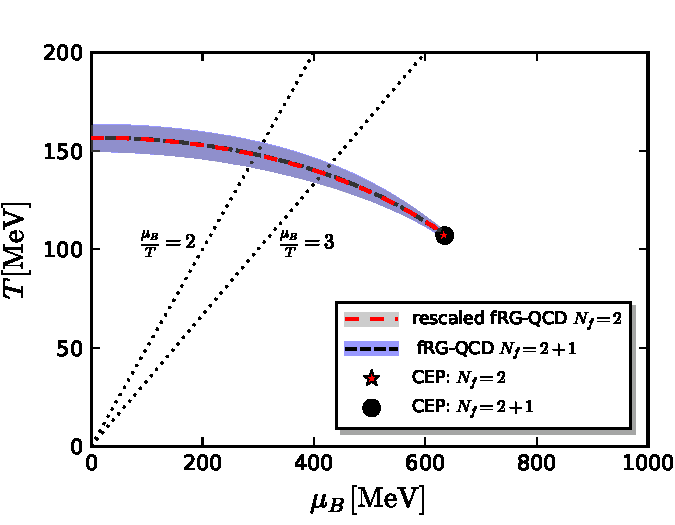
\includegraphics[width=0.45\textwidth]{QCD-scalematching}
		\caption{Phase boundaries of $N_f=2$-flavour QCD within a $N_f=2+1$-flavour scale matching at the crossover temperature and $\mu_B=0$.}\label{fig:QCD-scalematching}
	\end{figure}
	%%%%%%%%%%%%%%%%%%%%%%%%%%%%%
	%
	
	In summary, the convincing quantitative accuracy of the linear scale-matching analysis presented here for QCD also sustains its use in the LEFT within the present work. Note however, that we cannot simply take over the above QCD-relations for the present LEFT, which lacks the backcoupling of the glue-dynamics on both, large temperature and chemical potential physics. Still, the dominance of the leading order term $-\kappa \mu_B^2/T_c^2$ in the model reflects the same property in QCD. This allows us to employ a respective linear scale-matching for $\mu_B/T\lesssim 4$ as studied in the present work. 
	
	Analogously to QCD we choose the chiral crossover temperature at vanishing chemical potential, $(T,\mu_B)=(T_c,0)$ for fixing the scale factors $(c_{_T}, c_{\mu_B})$. Moreover, in the present work we are interested in fluctuations of conserved charges. Hence, instead of the renormalised condensate we use the kurtosis, or rather $R_{42}^B=\chi_4^B/\chi_2^B$ in \eq{eq:Rmn} for the determination of $c_T$: While the temperature-dependence of $R^{B}_{42}$ is a prediction of the LEFT, its absolute temperature has to be adjusted. This is done by minimising the $\chi^2$ of the difference between the lattice result and the LEFT-prediction as a function of the rescaled absolute temperature $c_T T_c$, leading us to 
	%
	\begin{align}
		c_{_{T}}=1.247(12)\,,\label{eq:c_T-LEFT}
	\end{align}
	%
	The respective result for $R_{42}$ is shown in \Fig{fig:T-adjust} in comparision to the lattice result from \cite{Borsanyi:2018grb}, and the two curves match quantitatively supporting the predictive power of the LEFT. 
	
	For the scale-matching of $\mu_B$ with the curvature $-\kappa \mu_B^2/T_c^2$ we have a plethora of results from state of the art functional approaches: $\kappa=0.0142(2)$ in  \cite{Fu:2019hdw}, $\kappa=0.0150(7)$ in \cite{Gao:2020qsj} and $\kappa=0.0147(5)$ in \cite{Gao:2020fbl}, the very recent update of \cite{Gao:2020fbl}. Lattice results are provided with $\kappa=0.015(4)$ in \cite{Bazavov:2018mes}, $\kappa=0.0149(21)$ in \cite{Bellwied:2015rza}, $\kappa=0.0153(18)$ in \cite{Borsanyi:2020fev}. Both, functional and lattice results agree within the respective (statistical and systematic) errors with a $\kappa\approx 0.015$. 
	
	%
	%%%%%%%%%%%%%%%%%%%%%%%%%%%%
	\begin{figure}[t]
		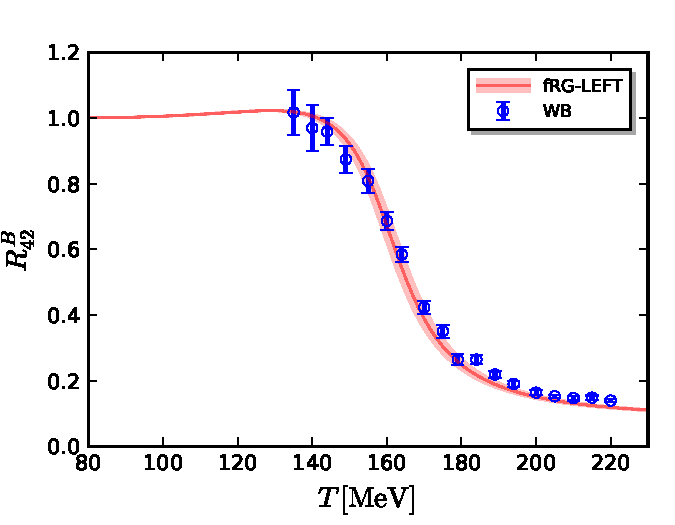
\includegraphics[width=0.45\textwidth]{T-adjust}
		\caption{Temperature scale maching LEFT-QCD with $R_{42}$ in \eq{eq:Rmn} with $c_{_{T}}=1.247(12)$, using the lattice results of \cite{Borsanyi:2018grb}. The $T/T_c$-dependence of $R_{42}$ is a prediction of the QCD-assisted LEFT used in the present work, and agrees quantitatively with the lattice results.}\label{fig:T-adjust}
	\end{figure}
	%%%%%%%%%%%%%%%%%%%%%%%%%%%%%
	%
	Having adjusted the temperature with results from the WB-collaboration, \cite{Bellwied:2015rza}, we use $\kappa=0.0153$ from \cite{Borsanyi:2020fev} for internal consistency. Note that the results presented here, do only change marginally, if using one a $\kappa$ in the range $\kappa=(0.042 - 0.053)$. Within the current LEFT including quantum, thermal and density fluctuations below $700$\,MeV, we obtain $\kappa_{_\textrm{LEFT}}=0.0193$. In comparison, $\kappa_{_{LEFT}}$ is large than the two-flavour QCD result in \cite{Fu:2019hdw} with $\kappa=0.0179(8)$. This reflects the lack of glue-dynamics in the LEFT. We 
	use this in the relation \eq{eq:cmuQCD} instead of $\kappa^{(N_f=2)}$, and arrive at  
	%
	\begin{align}
		c_{\mu_B}=c_{_{T}}\left(\frac{\kappa^{N_f=(2+1)}}{\kappa_{_{\textrm{LEFT}}}}\right)^{1/2}=1.110(66)\,, \label{eq:cmu-LEFT}
	\end{align}
	%
	with the LEFT-$c_{_T}$ from \eq{eq:c_T-LEFT}. 
	
	In summary, in this section we have utilised the scale-matching relations \eq{eq:rescale} between two- and 2+1-flavour QCD derived from the two- and 2+1-flavour QCD results in \cite{Fu:2019hdw}. These relations were applied to the present QCD-assisted LEFT. The scale matching was done with two observables relevant for the fluctuation physics studied here: $R^{B}_{42}$ as a function of $T$ and the curvature of phase boundary $\kappa$, both at vanishing chemical potential. This led us to the coefficients \eq{eq:c_T-LEFT} and \eq{eq:cmu-LEFT} 
	in \eq{eq:rescale}.
	
	
	%%%%%%%%%%%%%%%%%%%%%%%%%%%%%%%%%%%%%%%%%%%%%%%%%%%%%%%%%%%%%
	%%%%%%%%%%%%%%%%%%%%%%%%%%%%%%%%%%%%%%%%%%%%%%%%%%%%%%%%%%%%%
	
	\section{Thermodynamics and Hyper-order baryon number fluctuations}
	\label{sec:hyper-fluc}
	
	
	The thermodynamical potential density in the LEFT at finite temperature and nonzero baryon chemical potential is readily obtained from the effective action in \eq{eq:action} or rather from its integrated flow: we evaluate the effective action on the solution of the quantum equations of motion (EoMs). In the present work we consider only homogeneous (constant) solutions,  $(\sigma_\textrm{EoM}, A_{0,\textrm{EoM}})$ with
	%
	\begin{align}\label{eq:EoMs}
		\frac{\partial V(\rho, L,\bar L)}{\partial \sigma} =   \frac{\partial V(\rho, L,\bar L)}{\partial L} = \frac{\partial V(\rho, L,\bar L)}{\partial \bar L} =0\,, 
	\end{align}
	%
	while the quark fields vanish, $q,\bar q=0$. We also note that homogeneous have to be taken with a grain of salt for larger chemical potentials with $\mu_B/T\gtrsim 4$, see \cite{Fu:2019hdw}. With this preparations we are led to the grand potential 
	$\Omega[T,\mu_B]= V_{k=0}(\rho, L,\bar L)$, that is the effective potential, evaluated at vanishing cutoff scale $k=0$. It reads   
	%
	\begin{align}
		\Omega[T,\mu_B]=&V_{\mathrm{glue}}(L, \bar L)+V_{\mathrm{mat}}(\rho, L, \bar L)-c\sigma\,,\label{eq:Omega}
	\end{align}
	where the gluonic background field $A_0$ in \eq{eq:Vtotal} has been reformulated in terms of the Polyakov loop $L$ and its complex conjugate $\bar L$. As mentioned before, the matter sector of the effective potential is integrated out towards the IR limit $k=0$, for details see \hyperref[app:flowV]{App.~\ref{app:flowV}}, while the glue sector is independent of $k$, see \hyperref[app:gluepot]{App.~\ref{app:gluepot}}. The pressure of the system is directly related to the thermodynamical potential, as follows
	%
	\begin{align}
		p=&-\Omega[T,\mu_B]\,.\label{eq:pres}
	\end{align}
	%
	The generalized susceptibility of the baryon number $\chi^B_n$ is defined through the $n$-order derivative of the pressure w.r.t. the baryon chemical potential, to wit,
	%
	\begin{align}
		\chi_n^{B}&=\frac{\partial^n}{\partial (\mu_B/T)^n}\frac{p}{T^4}\,,\label{eq:suscept}
	\end{align}
	%
	and the ratio between the $m$- and $n$-th order susceptibilities is denoted as 
	%
	\begin{align}
		R_{mn}^{B}&=\frac{\chi_m^{B}}{\chi_n^{B}}\,.\label{eq:Rmn}
	\end{align}
	%
	The generalized susceptibilities are related to various cumulants of the baryon number distribution, which can be measured in heavy-ion collision experiments through the cumulants of its proxy, i.e., the net proton distribution, see, e.g. \cite{Luo:2017faz} for details. For the lowest four orders, one is led to
	%
	\begin{align}
		\chi^B_1=&\frac{1}{VT^3}\braket{N_B}\,,\quad \chi^B_2=\frac{1}{VT^3}\braket{(\delta N_B)^2}\,,\label{eq:chiB1}\\[2ex]
		\chi^B_3=&\frac{1}{VT^3}\braket{(\delta N_B)^3}\,,\\[2ex]
		\chi^B_4=&\frac{1}{VT^3}\Big(\braket{(\delta N_B)^4}-3\braket{(\delta N_B)^2}^2\Big)\,,\label{eq:chiB4}
	\end{align}
	%
	with $\braket{\cdots}$ denoting the ensemble average and $\delta N_B=N_B-\braket{N_B}$. Thus the mean value of the net baryon number of the system is given by $M=VT^3\chi_1^{B}$, the variance $\sigma^2=VT^3\chi_2^{B}$, skewness $S=\chi_3^{B}/(\chi_2^{B}\sigma)$, and the kurtosis $\kappa=\chi_4^{B}/(\chi_2^{B}\sigma^2)$, respectively.
	
	In this work emphasis is, however, put on the baryon number fluctuations of order higher than the fourth, i.e., $\chi_n^{B}$'s ($n>4$), which are named hyper-order baryon number fluctuations. As same as the low-order ones, the hyper-order susceptibilities are also connected to their respective cumulants, and their relations, taking the fifth through eighth ones for instance, are given as follows
	%
	\begin{align}
		\chi^B_5=&\frac{1}{VT^3}\Big(\braket{(\delta N_B)^5}-10\braket{(\delta N_B)^2}\braket{(\delta N_B)^3}\Big)\,,\\[2ex]
		\chi^B_6=&\frac{1}{VT^3}\Big(\braket{(\delta N_B)^6}-15\braket{(\delta N_B)^4}\braket{(\delta N_B)^2}\nonumber\\[2ex]
		&-10\braket{(\delta N_B)^3}^2+30\braket{(\delta N_B)^2}^3\Big)\,,
	\end{align}
	\begin{align}
		\chi^B_7=&\frac{1}{VT^3}\Big(\braket{(\delta N_B)^7}-21\braket{(\delta N_B)^5}\braket{(\delta N_B)^2}\nonumber\\[2ex]
		&-35\braket{(\delta N_B)^4}\braket{(\delta N_B)^3}\nonumber\\[2ex]
		&+210\braket{(\delta N_B)^3}\braket{(\delta N_B)^2}^2\Big)\,,\\[2ex]
		\chi^B_8=&\frac{1}{VT^3}\Big(\braket{(\delta N_B)^8}-28\braket{(\delta N_B)^6}\braket{(\delta N_B)^2}\nonumber\\[2ex]
		&-56\braket{(\delta N_B)^5}\braket{(\delta N_B)^3}-35\braket{(\delta N_B)^4}^2\nonumber\\[2ex]
		&+420\braket{(\delta N_B)^4}\braket{(\delta N_B)^2}^2\nonumber\\[2ex]
		&+560\braket{(\delta N_B)^3}^2\braket{(\delta N_B)^2}-630\braket{(\delta N_B)^2}^4\Big)\,.
	\end{align}
	%
	Different aspects of hyper-order fluctuations have been studied in mean-field approximations in the past, see e.g.\ \cite{Wagner:2009pm, Karsch:2010hm, Schaefer:2011ex}. However, due to the decisive role that non-perturbative quantum fluctuations play for these quantities, a treatment beyond mean-field, as in the present work, is necessary for their accurate description.
	
	
	%%%%%%%%%%%%%%%%%%%%%%%%%%%%%%%%%%%%%%%%%%%%%%%%%%%%%%%%%%%%%
	%%%%%%%%%%%%%%%%%%%%%%%%%%%%%%%%%%%%%%%%%%%%%%%%%%%%%%%%%%%%%
	
	\section{Numerical results and discussions}
	\label{sec:num}
	
	%
	%%%%%%%%%%%%%%%%%%%%%%%%%%%%%
	\begin{figure*}[t]
		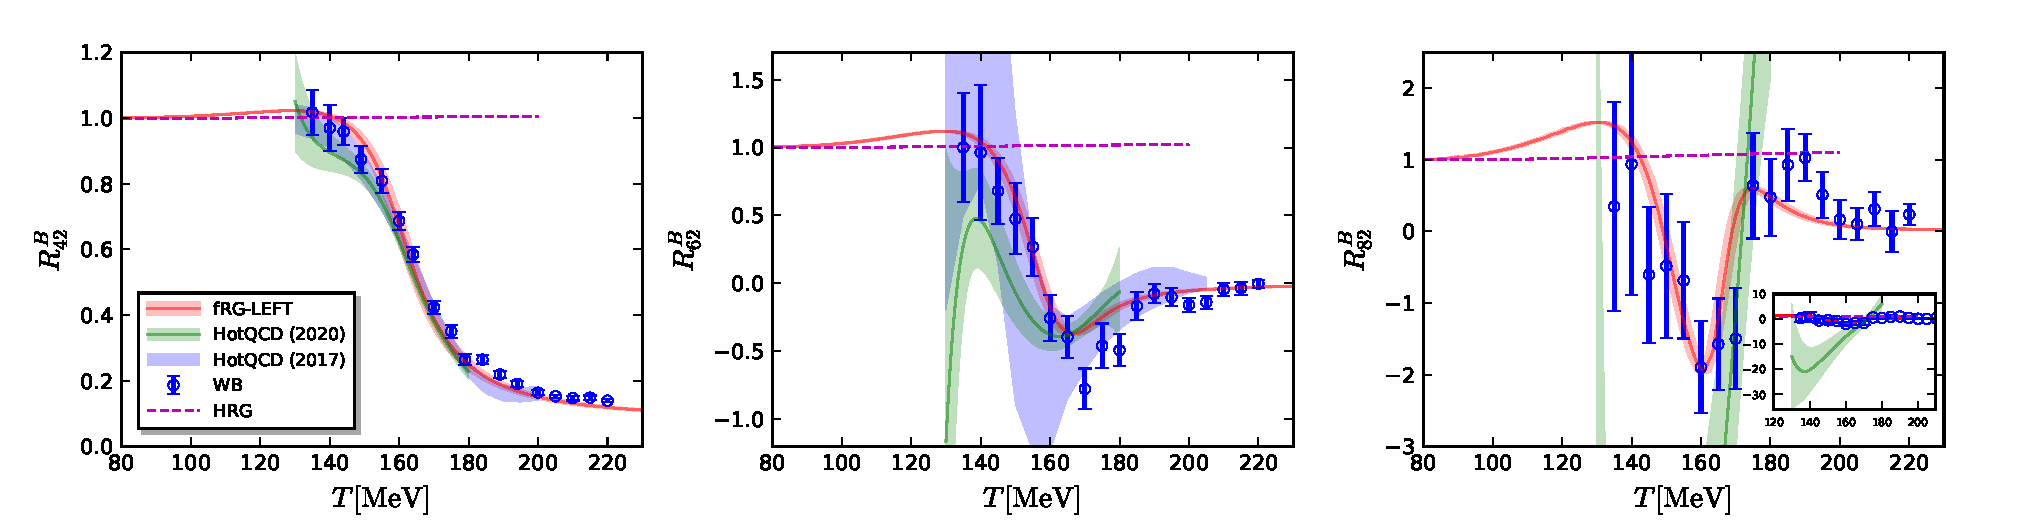
\includegraphics[width=1\textwidth]{R42R62R82-T-muB0}
		\caption{$R^{B}_{42}=\chi^{B}_{4}/\chi^{B}_{2}$ (left panel), $R^{B}_{62}=\chi^{B}_{6}/\chi^{B}_{2}$ (middle panel), and $R^{B}_{82}=\chi^{B}_{8}/\chi^{B}_{2}$ (right panel) as functions of the temperature with vanishing baryon chemical potential ($\mu_B=0$). Results obtained with the low energy effective theory within fRG approach are compared with lattice results from the HotQCD collaboration \cite{Bazavov:2017dus,Bazavov:2017tot,Bazavov:2020bjn} and the Wuppertal-Budapest collaboration \cite{Borsanyi:2018grb}. The inset in the plot of $R^{B}_{82}$ shows its zoom-out view.}\label{fig:R42R62R82-T-muB0}
	\end{figure*}
	%%%%%%%%%%%%%%%%%%%%%%%%%%%%%
	%
	
	%
	%%%%%%%%%%%%%%%%%%%%%%%%%%%%
	\begin{figure}[t]
		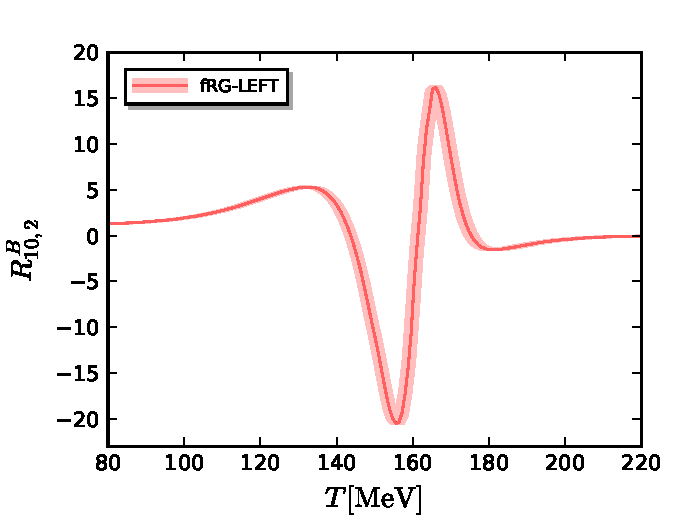
\includegraphics[width=0.45\textwidth]{R102-T-muB0}
		\caption{$R^{B}_{10,2}=\chi^{B}_{10}/\chi^{B}_{2}$ as a function of the temperature with $\mu_B=0$, predicted by the LEFT within the fRG approach.}\label{fig:R102-T-muB0}
	\end{figure}
	%%%%%%%%%%%%%%%%%%%%%%%%%%%%%
	%
	
	
	
	In this section we present and discuss our numerical results. At vanishing chemical potential the lower orders are compared to results from lattice calculations. We then discuss the implications of our predictions for the hyper-order baryon number fluctuations for decreasing collision energies (increasing chemical potential)  for heavy-ion collision experiments. 
	
	
	
	%%%%%%%%%%%%%%%%%%%%%%%%%%%%%%%%%%%%%%%%%%%%%%%%%%%%%%%%%%%%%
	\subsection{Hyper-order baryon number fluctuations}
	\label{subsec:hyper-order}
	
	%
	%%%%%%%%%%%%%%%%%%%%%%%%%%%%%
	%\begin{figure*}[t]
	%\centering
	%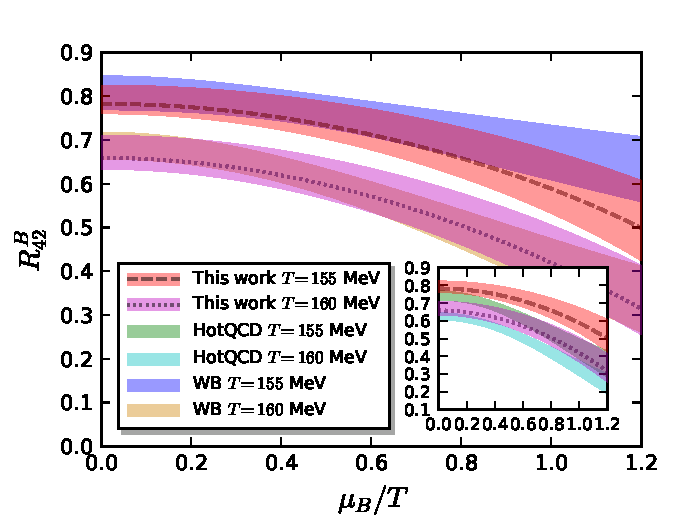
\includegraphics[width=0.85\columnwidth]{R42-muBoT} 
	%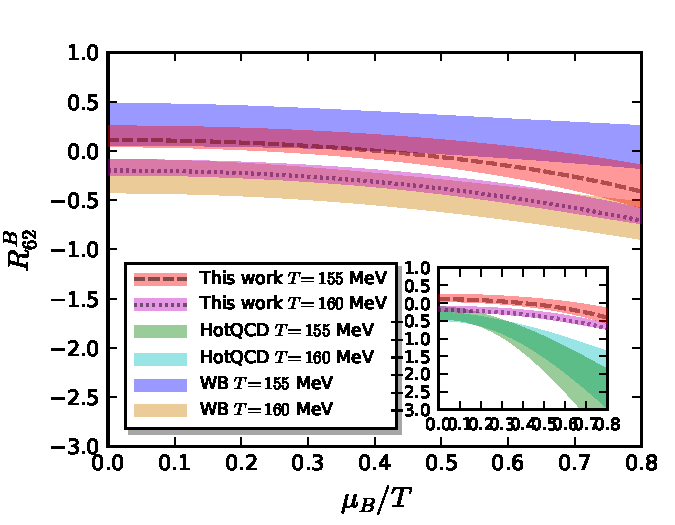
\includegraphics[width=0.85\columnwidth]{R62-muBoT} 
	%\caption{$R^{B}_{42}$ (left panel) and $R^{B}_{62}$ (right panel) as functions of $\mu_B/T$ with $T=155$ MeV and $T=160$ MeV. Calculation of LEFT within the fRG approach is compared with lattice QCD computations by the HotQCD collaboration \cite{Bazavov:2020bjn} and the Wuppertal-Budapest collaboration \cite{Borsanyi:2018grb}.
	%} \label{fig:R42R62-muBoT}
	%\end{figure*}
	%%%%%%%%%%%%%%%%%%%%%%%%%%%%%
	%
	
	%
	%%%%%%%%%%%%%%%%%%%%%%%%%%%%%
	\begin{figure*}[t]
		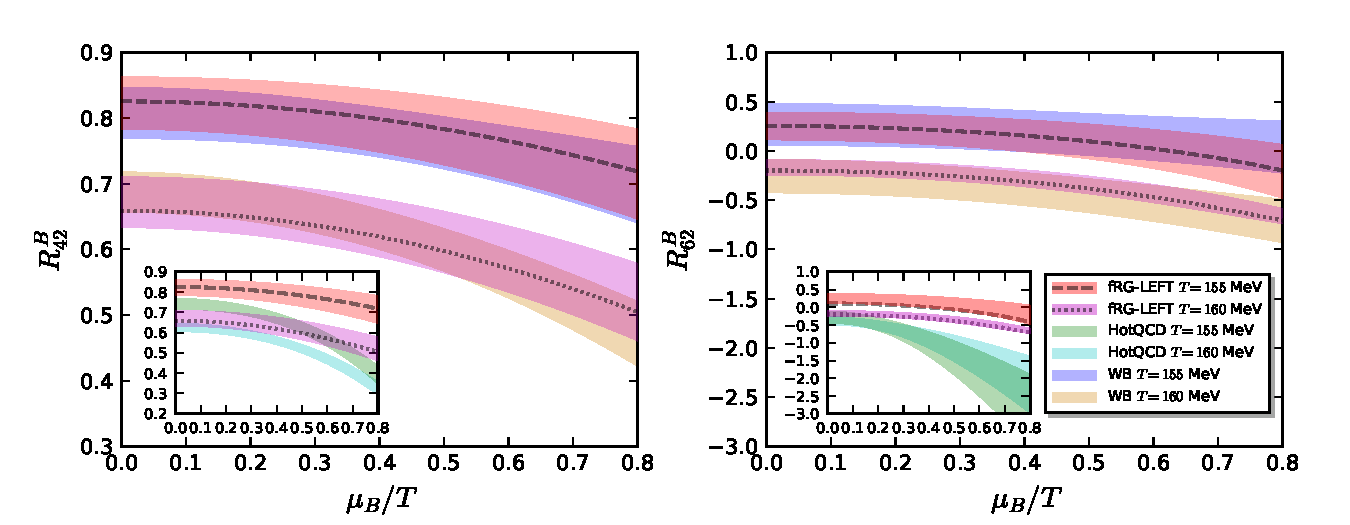
\includegraphics[width=0.9\textwidth]{R42R62-muBoT}
		\caption{$R^{B}_{42}$ (left panel) and $R^{B}_{62}$ (right panel) as functions of $\mu_B/T$ with $T=155$ MeV and $T=160$ MeV. Calculation of LEFT within the fRG approach is compared with lattice QCD by the HotQCD collaboration \cite{Bazavov:2020bjn} and the Wuppertal-Budapest collaboration \cite{Borsanyi:2018grb}. Note that the comparison of $R^{B}_{42}$ between HotQCD and LEFT is presented in the inlays, in order to improve the readability of presentation.}\label{fig:R42R62-muBoT}
	\end{figure*}
	%%%%%%%%%%%%%%%%%%%%%%%%%%%%%
	%
	
	%
	%%%%%%%%%%%%%%%%%%%%%%%%%%%%%
	\begin{figure*}[t]
		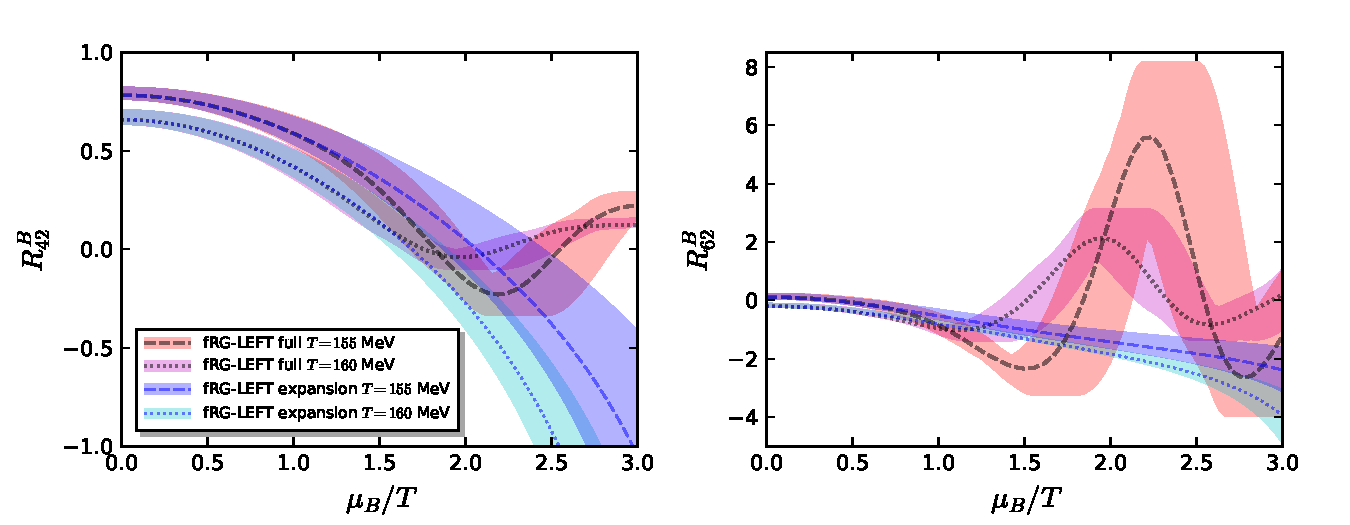
\includegraphics[width=0.9\textwidth]{R42R62expansion-muBoT}
		\caption{Comparison between the direct full calculation of baryon number fluctuations $R^{B}_{42}$ (left panel) and $R^{B}_{62}$ (right panel) via \Eq{eq:suscept} and the Taylor expansion in Eqs. (\ref{eq:chiB2Tay})  (\ref{eq:chiB4Tay})  (\ref{eq:chiB6Tay}). Both calculations are performed within the LEFT-fRG approach, and $R^{B}_{42}$, $R^{B}_{62}$ are plotted as functions of $\mu_B/T$ with $T=155$ MeV and $T=160$ MeV.}\label{fig:R42R62expansion-muBoT}
	\end{figure*}
	%%%%%%%%%%%%%%%%%%%%%%%%%%%%%
	%
	
	%
	%%%%%%%%%%%%%%%%%%%%%%%%%%%%%
	\begin{figure*}[t]
		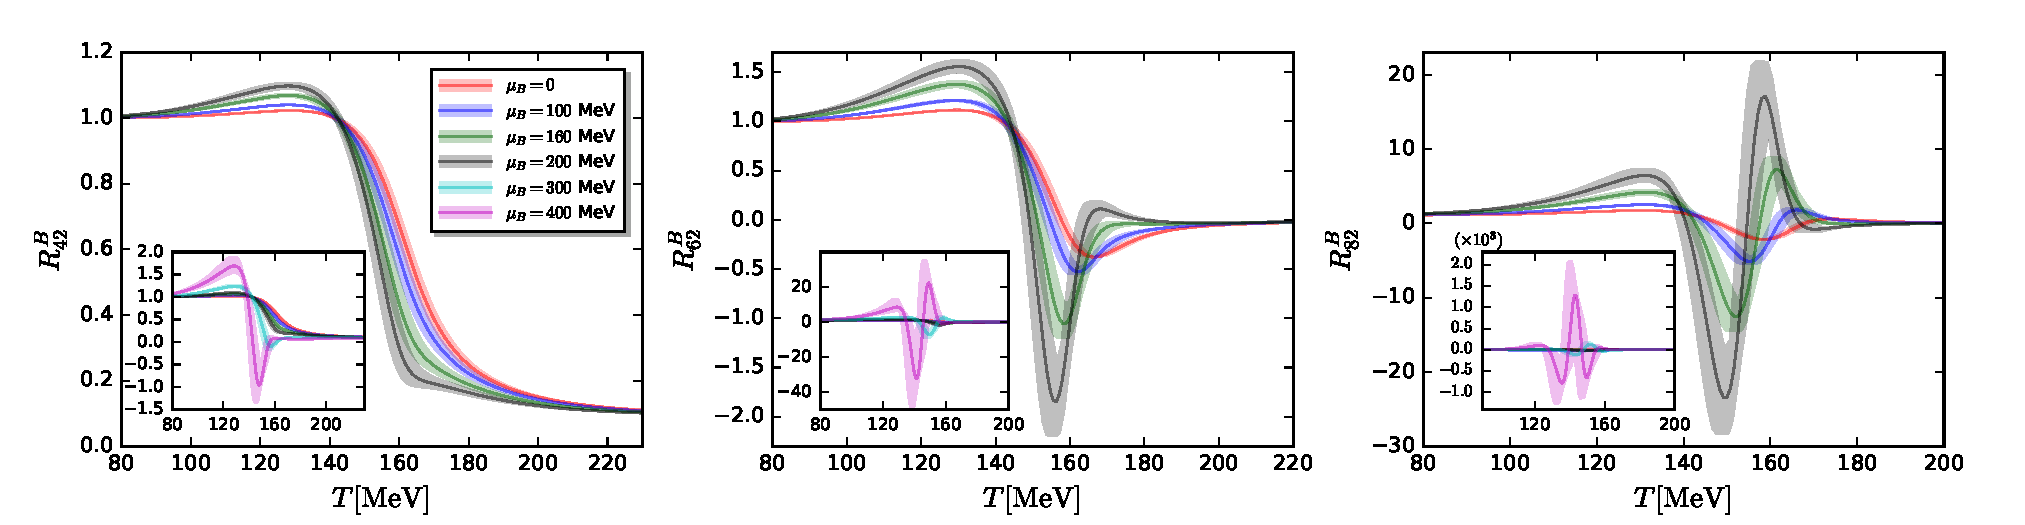
\includegraphics[width=1.\textwidth]{R42R62R82-T-muB0to400}
		\caption{$R^{B}_{42}$ (left panel), $R^{B}_{62}$ (middle panel), and $R^{B}_{82}$ (right panel) as functions of the temperature at several values of $\mu_B$, computed from LEFT within the fRG approach. Insets in each plot show their respective zoom-out view.}\label{fig:R42R62R82-T-muB0to400}
	\end{figure*}
	%%%%%%%%%%%%%%%%%%%%%%%%%%%%%
	%
	
	As we have discussed above, the LEFT has been calibrated by use of the curvature of phase boundary and the kurtosis of baryon number distribution as a function of $T$ with $\mu_B=0$, via a detailed comparison with recent lattice results. Consequently, one could use the LEFT to make predictions for the dependence of $R^{B}_{42}$ on the chemical potential, as well as the hyper-order baryon number fluctuations at finite temperature and density. In the middle and right panels of \Fig{fig:R42R62R82-T-muB0}, $R^{B}_{62}=\chi^{B}_{6}/\chi^{B}_{2}$ and $R^{B}_{82}=\chi^{B}_{8}/\chi^{B}_{2}$ are shown versus the temperature with vanishing $\mu_B$, respectively, and in the same way the LEFT and lattice QCD results are compared. Apparently, one observes that, with the increase of the order of fluctuations, errors of lattice calculation increase dramatically. Specifically, the eighth-order fluctuations $R^{B}_{82}$ obtained by the two collaborations show a significant quantitative difference, although they are roughly consistent with each other qualitatively. It is found that the predicted hyper-order baryon number fluctuations from the LEFT within the fRG, are in qualitative agreement with both lattice results, and even consistent with the Wuppertal-Budapest result quantitatively within the errors. We have also computed the hyper-order fluctuations within a simple hadron resonance gas model \cite{BraunMunzinger:2003zd} and found them to be essentially equal to one with only a very minor monotonic increase with $T$ for $T \lesssim 140$~MeV. This is in agreement with our findings. Moreover, we have also computed baryon number fluctuations of orders even up to the tenth in the LEFT, and the relevant result $R^{B}_{10,2}=\chi^{B}_{10}/\chi^{B}_{2}$ is presented in \Fig{fig:R102-T-muB0}, where the chemical potential is chosen to be vanishing. Note that no lattice results for the tenth-order fluctuation are available for the moment, and the dependence of $R^{B}_{10,2}$ on the temperature in \Fig{fig:R102-T-muB0} is a pure prediction by the LEFT within the fRG approach, which needs to be confirmed by other calculations, e.g., lattice QCD, in the future.
	
	To proceed, we consider the chemical potential dependence of baryon number fluctuations. Expanding the pressure in \Eq{eq:pres} in powers of $\hat{\mu}_{B}\equiv\mu_B/T$ around $\hat{\mu}_{B}=0$ , one is led to 
	%
	\begin{align}
		\frac{p}{T^4}&=\frac{p}{T^4}\Big|_{\hat{\mu}_{B}=0}+\sum_{i=1}^{\infty}\frac{\chi^B_{2i}|_{\hat{\mu}_{B}=0}}{(2i)!}\hat{\mu}_{B}^{2i}\,.\label{eq:cmu}
	\end{align}
	%
	Truncating the Taylor expansion above up to order of $\hat{\mu}_{B}^{8}$ and employing \Eq{eq:suscept}, we obtain the expanded baryon number fluctuations in the first several orders, to wit,
	%
	\begin{align}
		\chi^B_2\simeq&\chi^B_2|_{\hat{\mu}_{B}=0}+\frac{\chi^B_4|_{\hat{\mu}_{B}=0}}{2!}\hat{\mu}_{B}^{2}+\frac{\chi^B_6|_{\hat{\mu}_{B}=0}}{4!}\hat{\mu}_{B}^{4}\nonumber\\[2ex]
		&+\frac{\chi^B_8|_{\hat{\mu}_{B}=0}}{6!}\hat{\mu}_{B}^{6}\,,\label{eq:chiB2Tay}\\[2ex]
		\chi^B_4\simeq&\chi^B_4|_{\hat{\mu}_{B}=0}+\frac{\chi^B_6|_{\hat{\mu}_{B}=0}}{2!}\hat{\mu}_{B}^{2}+\frac{\chi^B_8|_{\hat{\mu}_{B}=0}}{4!}\hat{\mu}_{B}^{4}\,,\label{eq:chiB4Tay}\\[2ex]
		\chi^B_6\simeq&\chi^B_6|_{\hat{\mu}_{B}=0}+\frac{\chi^B_8|_{\hat{\mu}_{B}=0}}{2!}\hat{\mu}_{B}^{2}\,.\label{eq:chiB6Tay}
	\end{align}
	%
	In \Fig{fig:R42R62-muBoT} we show the lattice results $\chi^B_4/\chi^B_2$ and $\chi^B_6/\chi^B_2$ based on the Taylor expansion above, and the fluctuations at vanishing chemical potential, viz. $\chi^B_{i}|_{\hat{\mu}_{B}=0}$ ($i=2$, 4, 6, 8) and relevant results in \Fig{fig:R42R62R82-T-muB0}, from the HotQCD collaboration \cite{Bazavov:2020bjn} and the Wuppertal-Budapest collaboration \cite{Borsanyi:2018grb}. Moreover, $\chi^B_n$'s in \Eq{eq:suscept} could also be computed directly in the LEFT within the fRG approach, without resorting to the Taylor expansion, and the relevant results are presented in \Fig{fig:R42R62-muBoT} for comparison. Here we choose two values of the temperature, and as expected, the LEFT result for the dependence of $R^{B}_{42}$ and $R^{B}_{62}$ on the chemical potential, agrees with both lattice results qualitatively, and is even quantitatively consistent with the Wuppertal-Budapest result. Moreover, it is of high interest to investigate the convergence of Taylor expansion in Eqs. (\ref{eq:chiB2Tay}) (\ref{eq:chiB4Tay}) (\ref{eq:chiB6Tay}), via a comparison to the full calculation of baryon number fluctuations in \Eq{eq:suscept}. We have done both calculations in the LEFT-fRG approach, and the relevant results are shown in \Fig{fig:R42R62expansion-muBoT}. One observes that the Taylor expansion in Eqs. (\ref{eq:chiB2Tay})  (\ref{eq:chiB4Tay})  (\ref{eq:chiB6Tay}), where it is expanded up to $\chi^B_8$ at vanishing baryon chemical potential for the $\mu_B$-dependence of baryon number fluctuations of lower orders, agrees with the full calculation for $R^{B}_{42}$ with $\mu_B/T$ going up to 1.2, but the convergence upper bound for the higher-order fluctuation $R^{B}_{62}$ is decreased to $\sim$ 0.8. We find that the full calculation of $R^{B}_{62}$ with $\mu_B/T \gtrsim 1.0$ deviates from that of Taylor expansion significantly.
	
	In \Fig{fig:R42R62R82-T-muB0to400} $R^{B}_{42}$, $R^{B}_{62}$ and $R^{B}_{82}$ are depicted as functions of $T$ with several values of $\mu_B$, which are calculated in LEFT with the fRG approach. Relevant results in \Fig{fig:R42R62R82-T-muB0} for $\mu_B=0$ are presented as well, in order to highlight effects of the finite baryon chemical potential, whose value is increased from zero to 400 MeV. One observes that both the magnitude and error of the fluctuations, in particular the high-order ones, grow with the increasing chemical potential. Due to the rapid increase of error for very high-order fluctuations at large baryon chemical potential, e.g., $R^{B}_{82}$ with $\mu_B\gtrsim 200$ MeV, it is reasonable to expect that the LEFT is losing its capability of making predictions in these regimes.
	
	%\begin{table}[t]
	%  \begin{center}
	%    \begin{tabular}{|c ||c|c|c|c|c|c|c|c|c|}
	%    \hline & & & & & & & & & \\[-2ex]
	%    \hline & & & & & & & & & \\[-1ex]
	%    $\sqrt{s_{NN}}$ [GeV] & 200 & 62.4 & 54.4 & 39 & 27 & 19.6 & 14.5 & 11.5 & 7.7\\[1ex]
	%    \hline & & & & & & & & & \\[-2ex]
	%    ${\mu_B}_{_{CF}}$ [MeV] & 22 & 68 & 78 & 106 & 148 & 196 & 252 & 303 & 406\\[1ex]
	%    \hline & & & & & & & & & \\[-2ex]
	%    $T_{_{CF}}$ (I) [MeV] &158 & 158 & 158 & 158 & 157 & 156 & 153 & 150 & 138\\[1ex]
	%    \hline & & & & & & & & & \\[-2ex]
	%    $T_{c}$ [MeV] & 164 & 164 & 164 & 163 & 162 & 161 & 158 & 155 & 146\\[1ex]
	%    \hline & & & & & & & & & \\[-2ex]
	%    $T_{_{CF}}$ (II) [MeV] & 162 & 163 & 163 & 161 & 159 & 156 & 151 & 145 & 134\\[1ex]
	%    \hline
	%    \end{tabular}
	%    \caption{Chemical freeze-out parameters ${\mu_B}_{_{CF}}$ and $T_{_{CF}}$ (freeze-out: I, II) for different center-of-mass energies per nucleon pair $\sqrt{s_{\mathrm{NN}}}$. See text for details.}
	%    \label{tab:freeze-out-para}  
	%  \end{center}\vspace{-0.5cm}
	%\end{table}
	
	%
	%%%%%%%%%%%%%%%%%%%%%%%%%%%%%
	\begin{figure}[t]
		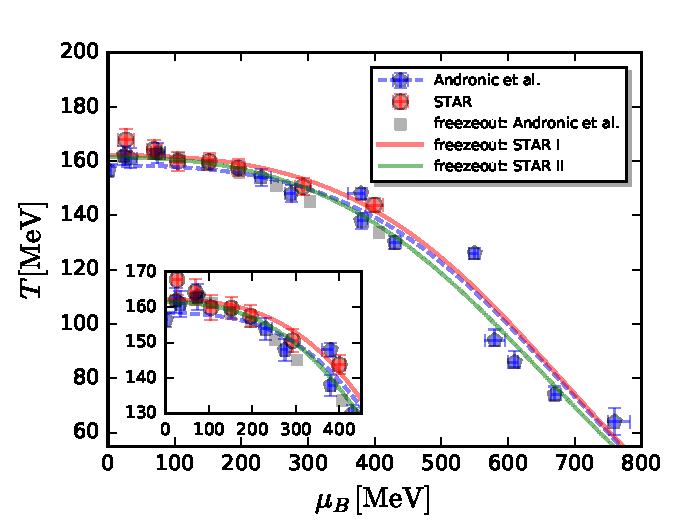
\includegraphics[width=0.48\textwidth]{phasediagram}
		\caption{Chemical freeze-out temperature and baryon chemical potential in the $T-\mu_B$ plane. The blue pentagons and red circles show the freeze-out data from Andronic {\it et al.} \cite{Andronic:2017pug} and STAR experiment \cite{Adamczyk:2017iwn}, respectively. The blue dashed line represents the parametrization of blue pentagons through Eqs. (\ref{eq:muBCFparatri}) and (\ref{eq:TCFparatri}). The red solid and green dotted lines show the parametrization of the STAR data based on all the seven data points, and only the four data points in the middle region ($100\,\mathrm{MeV}\lesssim\mu_B\lesssim 300\,\mathrm{MeV}$), respectively. The gray squares are obtained by interpolating the blue pentagons. The inlay zooms in the low-$\mu_B$ region.}\label{fig:phasediagram}
	\end{figure}
	%%%%%%%%%%%%%%%%%%%%%%%%%%%%%
	%
	
	%
	%%%%%%%%%%%%%%%%%%%%%%%%%%%%%
	\begin{figure}[t]
		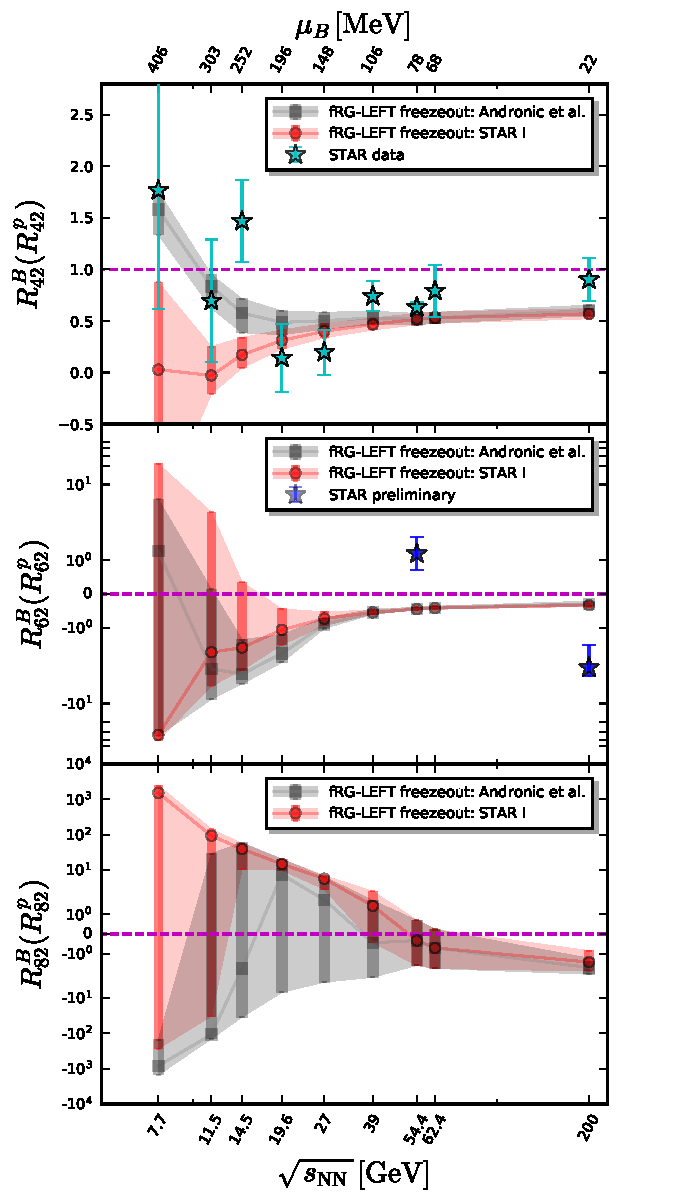
\includegraphics[width=0.45\textwidth]{Rm2-sqrtS}
		\caption{Baryon number fluctuations $R^{B}_{42}$ (top), $R^{B}_{62}$ (middle), and $R^{B}_{82}$ (bottom) as functions of the collision energy, calculated in LEFT within the fRG approach with the freeze-out parameters from Andronic {\it et al.} \cite{Andronic:2017pug} and STAR experiment \cite{Adamczyk:2017iwn}, where the parametrization of STAR freeze-out data is based on all the seven data points as shown in \Fig{fig:phasediagram} and is designated as freezeout: STAR I. Experimental data of cumulants from the STAR collaboration are also shown for comparison, where $R^{p}_{42}$ (top) are the kurtosis of the net-proton distributions measured in Au+Au central (0-5\%) collisions \cite{Adam:2020unf}, and $R^{p}_{62}$ (middle) is the preliminary result on the six-order cumulant of the net-proton distribution at $\sqrt{s_{\mathrm{NN}}}$=200 GeV and 54.4 GeV with centrality 0-40\% \cite{Nonaka:2020crv,Pandav:2020uzx}. The horizontal dashed lines indicate positions of unity for $R^{B}_{42}$($R^{p}_{42}$), zeros for $R^{B}_{62}$($R^{p}_{62}$) and $R^{B}_{82}$.}\label{fig:Rm2-sqrtS}\vspace{-0.5cm}
	\end{figure}
	%%%%%%%%%%%%%%%%%%%%%%%%%%%%%
	%
	
	%
	%%%%%%%%%%%%%%%%%%%%%%%%%%%%%
	\begin{figure}[t]
		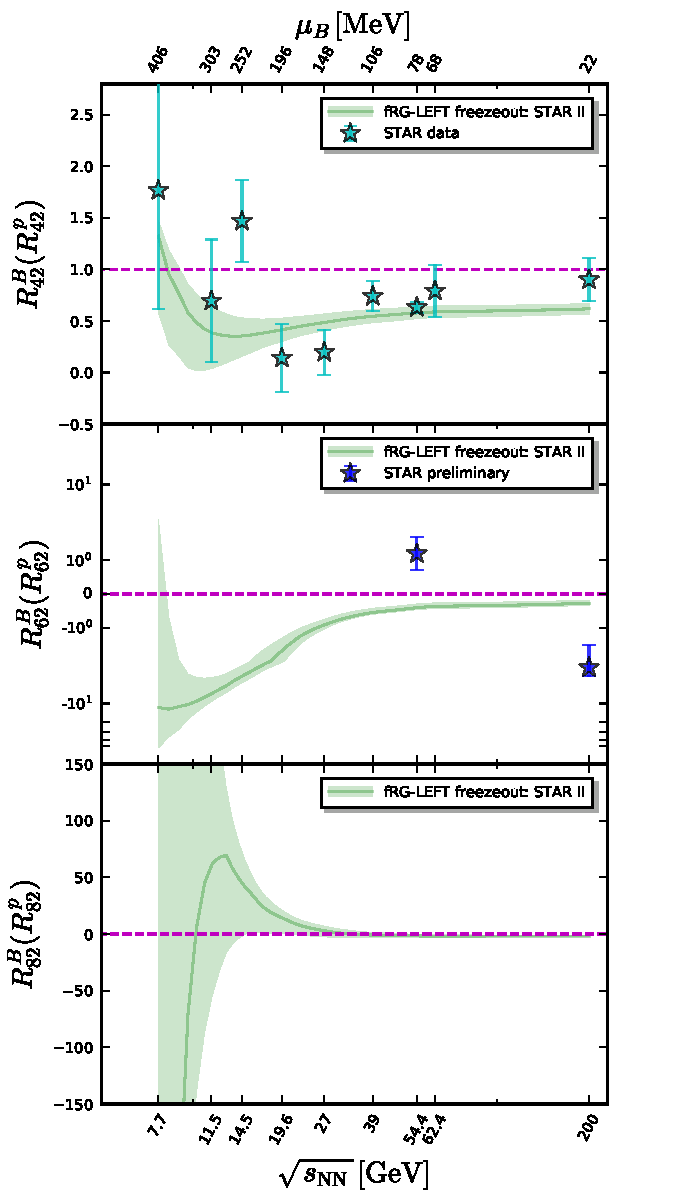
\includegraphics[width=0.45\textwidth]{Rm2-sqrtS2}
		\caption{Baryon number fluctuations $R^{B}_{42}$ (top), $R^{B}_{62}$ (middle), and $R^{B}_{82}$ (bottom) as functions of the collision energy, calculated in LEFT within the fRG approach with the freeze-out parameters from STAR experiment \cite{Adamczyk:2017iwn}, where the parametrization of STAR freeze-out data is based on only the four data points in the middle region ($100\,\mathrm{MeV}\lesssim\mu_B\lesssim 300\,\mathrm{MeV}$) as shown in \Fig{fig:phasediagram}, and is designated as freezeout: STAR II. Experimental data of cumulants from the STAR collaboration are also shown for comparison, where $R^{p}_{42}$ (top) are the kurtosis of the net-proton distributions measured in Au+Au central (0-5\%) collisions \cite{Adam:2020unf}, and $R^{p}_{62}$ (middle) is the preliminary result on the six-order cumulant of the net-proton distribution at $\sqrt{s_{\mathrm{NN}}}$=200 GeV and 54.4 GeV with centrality 0-40\% \cite{Nonaka:2020crv,Pandav:2020uzx}. The horizontal dashed lines indicate positions of unity for $R^{B}_{42}$($R^{p}_{42}$), zeros for $R^{B}_{62}$($R^{p}_{62}$) and $R^{B}_{82}$.}\label{fig:Rm2-sqrtS2}\vspace{-0.5cm}
	\end{figure}
	%%%%%%%%%%%%%%%%%%%%%%%%%%%%%
	%
	
	In the following we would like to confront theoretical predictions on the baryon number fluctuations with experimental measurement. Frankly speaking, a direct comparison between the theory and experiment is a challenging task, or even impossible within the setup in this work. This is due to the fact that experimental data are affected by many factors, e.g.,  acceptance of the detector such as the transverse momentum $p_T$ range, rapidity window and the centrality dependence \cite{Adamczyk:2013dal,Luo:2015ewa,Adam:2020unf,Nonaka:2020crv,Pandav:2020uzx}, cf. also \cite{Luo:2017faz,Adamczyk:2017iwn} for more details, volume fluctuations \cite{Luo:2013bmi}, global baryon number conservation \cite{Braun-Munzinger:2016yjz,Vovchenko:2020tsr}, resonance decays \cite{Nahrgang:2014fza}, etc. They constitute the non-critical contributions to fluctuation observables in experiments, and pinning down their contributions plays a pivotal role in identifying the critical signals in the BES experiment. Additionally, due to critical slowing down, nonequilibrium effects become important in the vicinity of the CEP \cite{Berdnikov:1999ph}, which necessitates a theoretical description of the dynamics of critical fluctuations. For more details about recent progress on the dynamics of critical fluctuations in QCD, see \cite{Bluhm:2020mpc} and references therein. We emphasise, however, that the present results are well outside the critical region of the present QCD-assisted LEFT, and therefore not subject to critical dynamics. 
	
	In this work we will not take into account the non-critical and dynamical effects discussed above when the theoretical results are confronted with experiments, but rather assume that the measured cumulants of the net-proton multiplicity distribution at a given collision energy, with other collision parameters e.g., the centrality and rapidity range fixed, is in one-by-one correspondence to the calculated fluctuations in \Eq{eq:suscept} with one value of $T$ or $\mu_B$. It is reasonable to attribute the values of $T$ and $\mu_B$ to be the ones when the chemical freeze-out occurs, viz. $T_{_{CF}}$ and ${\mu_B}_{_{CF}}$. Such an approach for the comparison is usually employed in fluctuation studies of equilibrium QCD matter within functional methods or lattice simulations \cite{Fu:2015amv,Isserstedt:2019pgx,Bazavov:2020bjn}. Note, however, that because of the reasons we have outlined above, results of comparison between the theory and experiment within this simplified approach should be taken with a grain of salt. In this work we adopt the freeze-out temperature and baryon chemical potential in \cite{Andronic:2017pug} and in STAR experiment \cite{Adamczyk:2017iwn}, which are shown in \Fig{fig:phasediagram} by the blue pentagons and red circles, respectively. They are both obtained from the analysis of hadron yields in the statistical hadron resonance gas model, see aforementioned references for more details. The freeze-out data in \cite{Andronic:2017pug} has also been parameterized as functions of the collision energy as follows
	%
	\begin{align}
		{\mu_B}_{_{CF}}&=\frac{a}{1+0.288\sqrt{s_{\mathrm{NN}}}},\label{eq:muBCFparatri}
	\end{align}
	%
	with $a=1307.5$ MeV, and
	%
	\begin{align}
		T_{_{CF}}&=\frac{T^{lim}_{_{CF}}}{1+\exp\big(2.60-\ln(\sqrt{s_{\mathrm{NN}}})/0.45\big)},\label{eq:TCFparatri}
	\end{align}
	%
	with $T^{lim}_{_{CF}}=158.4$ MeV. And this parametrization is depicted in \Fig{fig:phasediagram} by the blue dashed line. We use the same parametrization functions in Eqs. (\ref{eq:muBCFparatri}) and (\ref{eq:TCFparatri}) to fit the freeze-out data in STAR experiment, i.e., the red circle points in \Fig{fig:phasediagram}. Two parametrization curves are obtained: the red solid line and the green dotted one, where the former takes all the seven data points into account, while the latter only uses the four data points in the middle region ($100\,\mathrm{MeV}\lesssim\mu_B\lesssim 300\,\mathrm{MeV}$) for the fitting. The freeze-out curves of the red solid and green dotted lines in \Fig{fig:phasediagram} are labelled as freezeout: STAR I/II, respectively. The reason why we remove the first two data points in the low $\mu_B$ regime and the last one at $\mu_B\sim 400$ MeV in the parametrization of freezeout: STAR II, is due to the fact that the first two points are apparently higher than others and also a general consideration that the freeze-out curve in the plane of $T$-$\mu_B$ should be convex. One can see that, after these three data points are removed, the freeze-out line of STAR II moves down a bit to lower temperature in comparison to that of STAR I, which is more pronounced when $\mu_B\gtrsim 200$ MeV. 
	
	In \Fig{fig:Rm2-sqrtS} we show the dependence of baryon number fluctuations $R^{B}_{42}$, $R^{B}_{62}$, and $R^{B}_{82}$ on the center-of-mass collision energy, which is calculated in the LEFT within the fRG approach with the freeze-out parameters from Andronic {\it et al.} \cite{Andronic:2017pug} and the freeze-out line of STAR I. Note that the freeze-out data from Andronic {\it et al.} are used through direct interpolation, and the resulting results are shown in \Fig{fig:phasediagram} by the gray squares. The theoretical results are also confronted with experimental measurement of cumulants of the net-proton distributions in the beam energy scan experiments from the STAR collaboration. The kurtosis of the net-proton distributions $R^{p}_{42}$ are measured in Au+Au collisions with centrality 0-5\%, transverse momentum range $0.4< p_T\,(\mathrm{GeV}/c)\,<2.0$, and rapidity $|y|<0.5$, cf. \cite{Adam:2020unf} for more details. Moreover, preliminary results for the six-order cumulant of the net-proton distribution $R^{p}_{62}$ are also presented in the middle plot of \Fig{fig:Rm2-sqrtS}, which are obtained at two values of the collision energy, i.e., $\sqrt{s_{NN}}$=200 GeV and 54.4 GeV with centrality 0-40\% \cite{Nonaka:2020crv,Pandav:2020uzx}. In \Fig{fig:Rm2-sqrtS2} we show a similar calculation but with the freeze-out line of STAR II, and compare it with the experiment measurement as well.
	
	As shown in \Fig{fig:Rm2-sqrtS} as well as \Fig{fig:Rm2-sqrtS2}, the theoretical result of the fourth-order fluctuations calculated in the fRG-LEFT approach with the freeze-out data from Andronic {\it et al.}, as shown by the gray squares and band, is in qualitative agreement with the experimental measurement of the kurtosis of net-proton distributions.  In particular, a nonmonotonic behavior in the low collision energy regime, below $\sim 20$ GeV, is found in the fRG calculation. The nonmonotonic behavior is also found in the results with the freezeout parametrizations STAR I and STAR II. The nonmonotonic behavior from STAR I is significantly weaker than the others because the freeze-out temperature of STAR I is larger than the two others, in particular in the region of high $\mu_B$, as shown in \Fig{fig:phasediagram}. This shows that even small variations in the freeze-out temperature have a substantial effect on the fluctuations. The underlying reason is that the freezout happens in or close to the crossover region, where the fluctuations vary significantly, see \Fig{fig:R42R62R82-T-muB0to400}.
	
	It is important to emphasise that the strong nonmonotonic behavior of our results for $R^{B}_{42}$ at small  beam-energies in the top panel of \Fig{fig:Rm2-sqrtS} has nothing to do with critical physics. In our model, the CEP is at significantly larger $\mu_B$ \coljan{ \bf Please provide the CEP location of our LEFT!}, and it is well established that the critical region is only very small, see e.g.\ \cite{Schaefer:2006ds}. This is a crucial point since a nonmonotonic behavior, e.g., of $R^{B}_{42}$ as a function of $\sqrt{s_{NN}}$ has been proposed as an experimental signature of a CEP \cite{Stephanov:1999zu, Stephanov:2011pb}. However, these works only show that critical physics is sufficient for nonmonotonic behavior. Our results unequivocally demonstrate that \emph{not only} critical behavior  leads to nonmonotonic behavior, it \emph{also} occurs at finite $\mu_B$ far away from a CEP. In the present case, it is a result of two effects. First, correlations are enhanced since the chiral crossover becomes sharper with increasing $\mu_B$. This leads to stronger nonmonotonic behavior of $R^{B}_{42}$ as a function of $T$ (see \Fig{fig:R42R62R82-T-muB0to400}.). Second, the freeze-out temperature is shifted away from the pseudocritical temperature towards small beam-energies, thereby probing different regimes of the cumulants.
	
	
	Moreover, the nonmonotonic behavior is also observed in the sixth-order and eighth-order baryon number fluctuations as functions of the collision energy, as shown in the center and bottom panel of \Fig{fig:Rm2-sqrtS} and \Fig{fig:Rm2-sqrtS2}. 
	\colfab{The discussion of the previous paragraph clearly also applies here.}
	However, it should be noted that the error of our results increases significantly in the low energy region. These errors include the systematic error of the fRG-LEFT approach, which stem from the uncertainty in the matching of the in-medium scales of the LEFT and QCD, encoded in the coefficients $c_{_{T}}$ and $c_{\mu}$ in \Eq{eq:rescale}.
	For $\sqrt{s_{NN}}$=200 GeV and 54.4 GeV we can compare our results for $R^{B}_{62}$ to preliminary STAR data \cite{Nonaka:2020crv,Pandav:2020uzx}. As opposed to $R^{B}_{42}$, we find large deviations between our and the experimental results. At the highest beam energy, $\sqrt{s_{NN}}$=200 GeV, we at least agree qualitatively in that $R^{B}_{42}$ is negative.
	
	
	
	
	
	%%%%%%%%%%%%%%%%%%%%%%%%%%%%%%%%%%%%%%%%%%%%%%%%%%%%%%%%%%%
	%%%%%%%%%%%%%%%%%%%%%%%%%%%%%%%%%%%%%%%%%%%%%%%%%%%%%%%%%%%
	
	\section{summary and conclusions}
	\label{sec:summary}
	
	\coljan{\bf summary not touched yet}
	In this work we have studied the baryon number fluctuations in the LEFT within the fRG approach, putting emphasis on the hyper-order ones. The order of baryon number fluctuations has been computed up to the $10^{\mathrm{th}}$ order for the first time beyond mean-field. In our calculations, quantum, thermal and density fluctuations are successively encoded through the evolution of flow equations. Moreover, nontrivial dispersion relation for the quark and meson fields, momentum scale dependence of the quark-meson scattering, and fluctuations of Polyakov loop are also taken into account in this work.
	
	The scale between the LEFT and QCD is matched via a comparison of the temperature dependence of $R^{B}_{42}=\chi^{B}_{4}/\chi^{B}_{2}$ at vanishing $\mu_B$ between the LEFT and lattice results, as well as a comparison of the curvature of phase boundary. Accordingly, it allows us to employ the LEFT within the fRG approach to make predictions for the $\mu_B$-dependence of $R^{B}_{42}$, and the hyper-order baryon number fluctuations at finite temperature and density. In turn, relevant predictions of LEFT are compared with results of lattice QCD simulations. We find that the $T$- and $\mu_B$-dependence of hyper-order baryon number fluctuations, $\mu_B$-dependence of $R^{B}_{42}$ obtained in the fRG-LEFT approach, are in quantitative accordance with the lattice results by the Wuppertal-Budapest collaboration within errors. There is still a sizable quantitative deviation in comparison to relevant results by the HotQCD collaboration, but a qualitative consistency is observed.
	
	Furthermore, by employing the commonly used chemical freeze-out temperature and baryon chemical potential from Andronic {\it et al.} \cite{Andronic:2017pug} and STAR experiment \cite{Adamczyk:2017iwn}, we obtain baryon number fluctuations $R^{B}_{42}$, $R^{B}_{62}$, and $R^{B}_{82}$ as functions of the collision energy, which are compared with experimental measurements of the kurtosis and sixth-order cumulants of the net-proton distributions from the STAR collaboration. Remarkably, the dependence of the fourth-order baryon number fluctuation $R^{B}_{42}$ on the collision energy obtained in the fRG-LEFT approach, is qualitative consistent with the experimental measured dependence of the kurtosis of net-proton distributions on the collision energy for central collisions. And a nonmonotonic behavior of $R^{B}_{42}$ as a function of $\sqrt{s_{\mathrm{NN}}}$ is found in the fRG calculation. It should, however, be cautioned that errors of $R^{B}_{42}$ and $R^{B}_{62}$ increase significantly in the low collision energy region. And when the order of baryon number fluctuations is increased up to the $8^{\mathrm{th}}$, the theoretical calculation with current setup is losing its capability of making predictions, as a consequence of the significant errors of $R^{B}_{82}$ for large range of collision energy. Apparently, in order to improve on the computation in this work in the future, and decrease the errors of calculated baryon number fluctuations, especially in the low collision energy regime, on the one hand, the systematic errors of theoretical calculations should be reduced, and on the other hand, chemical freeze-out data with high precision are highly required.
	
	
	
	%%%%%%%%%%%%%%%%%%%%%%%%%%%%%%%%%%%%%%%%%%%%%%%%%%%%%%%%%%%
	%%%%%%%%%%%%%%%%%%%%%%%%%%%%%%%%%%%%%%%%%%%%%%%%%%%%%%%%%%%
	
	\begin{acknowledgments}
		
		We thank Nu Xu for discussions. The work was supported by the National Natural Science Foundation of China under Contracts Nos. 11775041. The work is also supported by EMMI, the BMBF grant 05P18VHFCA, and by the DFG Collaborative Research Centre SFB 1225 (ISOQUANT). This work is supported by Deutsche Forschungsgemeinschaft (DFG, German Research Foundation) under Germany’s Excellence Strategy EXC-2181/1 - 390900948 (the Heidelberg STRUCTURES Cluster of Excellence).
		
		
	\end{acknowledgments}
	
	%%%%%%%%%%%%%%%%%%%%%%%%%%%%%%%%%%%%%%%%%%%%%%%%%%%%%%%%%%%%%
	%%%%%%%%%%%%%%%%%%%%%%%%%%%%%%%%%%%%%%%%%%%%%%%%%%%%%%%%%%%%%
	
	\appendix
	
	\section{The fRG-approach to QCD \& LEFTs}\label{app:fRG}
	
	The flow equation for QCD describes the evolution of its effective action with the infrared cutoff scale $k$. This formulation with \textit{dynamical hadronisation}, \cite{Gies:2001nw, Gies:2002hq, Pawlowski:2005xe, Floerchinger:2009uf, Fu:2019hdw} has been developped in \cite{Mitter:2014wpa,Braun:2014ata,Cyrol:2017ewj,Fu:2019hdw}, its current form has been described and further developped in \cite{Fu:2019hdw}. The derivation of the respective flow equation is detailed there, and reads, 
	%
	\begin{align}
		\partial_t\Gamma_k[\Phi]=&\frac{1}{2}\mathrm{Tr}\Big(G_{AA,k}\partial_t R_{A,k}\Big)-\mathrm{Tr}\Big(G_{c\bar c,k}\partial_t R_{c,k}\Big)\nonumber\\[2ex]
		&-\mathrm{Tr}\Big(G_{q\bar q,k}\partial_t R_{q,k}\Big)+\frac{1}{2}\mathrm{Tr}\Big(G_{\phi\phi,k}\partial_t R_{\phi,k}\Big)\,,\label{eq:QCDflow}
	\end{align}
	%
	with $\Phi=(A, c, \bar c, q,\bar q,\phi)$, where $G$'s and $R$'s are the propagators and regulators of different fields, respectively. Diagrammatically it is depicted in \Fig{fig:QCD_equation}. For more works on QCD-flows at finite temperature and density see \cite{Braun:2007bx,Braun:2008pi,Braun:2009gm,Mitter:2014wpa,Braun:2014ata,Cyrol:2016tym,Cyrol:2017ewj,Cyrol:2017qkl,Fu:2019hdw,Braun:2020ada}, for reviews on QCD and LEFTs for QCD see    \cite{Berges:2000ew,Pawlowski:2005xe,Schaefer:2006sr,Gies:2006wv,Rosten:2010vm,Braun:2011pp,Pawlowski:2014aha,Dupuis:2020fhh}.
	
	For scales $k\lesssim 1$ GeV, the gluon decouples due to its confinement-related mass gap from the system. The dynamics is taken over by the emergent composite degrees of freedom, e.g. mesons, in particular the $\pi$ meson, which is in essence the Goldstone boson related to the spontaneously breaking chiral symmetry in the low energy QCD, and is the lightest hadron of mass $\sim 140$ MeV in the vacuum. In this regime, the flow equation of the effective action in \Eq{eq:QCDflow} is reduced to 
	%
	\begin{align}
		\partial_t\Gamma_k[\Phi]=&-\mathrm{Tr}\Big(G_{q\bar q,k}\partial_t R_{q,k}\Big)+\frac{1}{2}\mathrm{Tr}\Big(G_{\phi\phi,k}\partial_t R_{\phi,k}\Big)\,,\label{eq:LEFTflow}
	\end{align}
	%
	where $R_{q,k}$ and $R_{\phi,k}$ are the regulators for the quark and meson fields, respectively. The full propagators in \eq{eq:LEFTflow} read
	%
	\begin{align}
		G_{q\bar q/\phi\phi,k}=&\left(\frac{1}{\Gamma^{(2)}_k[\Phi]+R_k}\right)_{q\bar q/\phi\phi}\,,\label{}
	\end{align}
	%
	with $\Gamma^{(2)}_k[\Phi]=\delta^2\Gamma_k[\Phi]/(\delta \Phi_{i_1}\delta \Phi_{i_2})$, where different species of fields are distinguished with the help of the subscripts in $\Phi_{i_1/i_2}$. 
	
	In this work we employ  $3d$-flat or Litim regulators \cite{Litim:2000ci, Litim:2001up, Litim:2006ag}, 
	\begin{align}\nonumber 
		R_{\phi,k}(q_0,\bm{q})&=Z_{\phi,k}\bm{q}^2 r_B(\bm{q}^2/k^2)\,, \\[2ex] 
		R_{q,k}(q_0,\bm{q})&=Z_{q,k}i\bm{\gamma} \cdot \bm{q} r_F(\bm{q}^2/k^2)\,, \label{eq:Rk}
	\end{align} 
	with 
	\begin{align}\nonumber 
		r_B(x)&=\left( \frac{1}{x}-1 \right)\Theta(1-x)\,,\\[2ex] 
		r_F(x)&=\left( \frac{1}{\sqrt{x}}-1 \right)\Theta(1-x)\,,  \label{eq:rk}
	\end{align} 
	where $\Theta(x)$ denotes the Heaviside step function. 
	
	Inserting the effective action \eq{eq:action} into the flow equation \eq{eq:LEFTflow}, one is led to the flow equation for the effective potential of the matter sector, as follows
	%
	\begin{align}
		\partial_t V_{\mathrm{mat},k}(\rho)=&\frac{k^4}{4\pi^2} \bigg [\big(N^2_f-1\big) l^{(B,4)}_{0}(\tilde{m}^{2}_{\pi,k},\eta_{\phi,k};T)\nonumber\\[2ex]
		&+l^{(B,4)}_{0}(\tilde{m}^{2}_{\sigma,k},\eta_{\phi,k};T)\nonumber\\[2ex]
		&-4N_c N_f l^{(F,4)}_{0}(\tilde{m}^{2}_{q,k},\eta_{q,k};T,\mu)\bigg]\,, \label{eq:flowV}
	\end{align}
	%
	where the threshold functions $l^{(B/F,4)}_{0}$ as well as other threshold functions in the following can be found in e.g., \cite{Fu:2019hdw,Yin:2019ebz}, and the dimensionless renormalized quark and meson masses read
	%
	\begin{align}
		\tilde{m}^{2}_{q,k}=&\frac{h^{2}_{k}\rho}{2k^2Z^{2}_{q,k}}\,, \qquad \tilde{m}^{2}_{\pi,k}=\frac{V'_{\mathrm{mat},k}(\rho)}{k^2 Z_{\phi,k}}\,, \\[2ex]
		\tilde{m}^{2}_{\sigma,k}=&\frac{V'_{\mathrm{mat},k}(\rho)+2\rho V''_{\mathrm{mat},k}(\rho)}{k^2 Z_{\phi,k}}\,.\label{}
	\end{align}
	%
	
	The anomalous dimensions for the quark and meson fields in \Eq{eq:flowV} are defined as
	%
	\begin{align}
		\eta_{q,k}&=-\frac{\partial_t Z_{q,k}}{Z_{q,k}}\,,\qquad
		\eta_{\phi,k}=-\frac{\partial_t Z_{\phi,k}}{Z_{\phi,k}}\,,
	\end{align}
	%
	respectively. Accordingly, projecting the flow in \Eq{eq:LEFTflow} onto the one-particle irreducible (1PI) two-point function of the meson, it is readily obtained that 
	%
	\begin{align}
		\eta_{\phi,k}&=-\frac{1}{3Z_{\phi,k}}\delta_{ij}\frac{\partial}{\partial (|\bm{p}|^2)}\frac{\delta^2 \partial_t \Gamma_k}{\delta \pi_i(-p) \delta \pi_j(p)}\Bigg|_{\substack{p_0=0\\ \bm{p}=0}}\,,\label{eq:etaphi}
	\end{align}
	%
	where the spacial component is employed. Note that in the case of finite temperature and density, the $\mathrm{O}(4)$ rotation symmetry in the 4-$d$ Euclidean space is broken, and as a matter of fact, the mesonic anomalous dimension extracted above is different from that projected onto the temporal component. In another word, $\eta_{\phi,k}$ is split into $\eta_{\phi,k}^{\perp}$ and $\eta_{\phi,k}^{\parallel}$, which are transverse and longitudinal to the heat bath, respectively, at finite temperature and density. The influences of the splitting of $\eta_{\phi,k}$ on the thermodynamics and baryon number fluctuations have been investigated in detail \cite{Yin:2019ebz}, and it has been found that the impact is small. Therefore, it is reasonable to disregard the splitting of anomalous dimensions, and $\eta_{\phi,k}=\eta_{\phi,k}^{\perp}=\eta_{\phi,k}^{\parallel}$, as well as that for the quark anomalous dimension in the following, is assumed throughout this work. In the same way, the quark anomalous dimension is obtained by projecting the relevant flow onto the vector channel of the 1PI quark-antiquark correlation function, as follows
	%
	\begin{align}
		\eta_{q}&=\frac{1}{4 Z_{q,k}}\nonumber\\[2ex]
		&\times\mathrm{Re}\left[\frac{\partial}{\partial (|\bm{p}|^2)}\mathrm{tr}
		\left(i \bm{\gamma}\cdot\bm{p}\left(-\frac{\delta^2}{\delta\bar{q}(p)
			\delta q(p)}\partial_t \Gamma_k\right)\right)\right]\Bigg|_{\substack{p_{0,ex}\\ \bm{p}=0}}\,,  \label{eq:etapsi}
	\end{align}
	%
	where the external spacial momentum is chosen to be zero as same as the mesonic one, since the vanishing momentum is most relevant to the flow of effective potential in \Eq{eq:flowV}. Note that the lowest mode of the fermionic Matsubara frequency is nonvanishing and we designate it here as $p_{0,ex}$, to be described in \app{app:flowV}. Moreover, the expression in the square bracket in \eq{eq:etapsi} is complex-valued, rather than real, when the chemical potential is nonzero. This artifact stems from the naive truncation of the external frequency, which is resolved through a resummation of the external frequency of the quark propagator \cite{Fu:2016tey}. The flow equation of the Yukawa coupling is readily obtained via the projection of the 1PI quark-antiquark correlation function on the scalar channel, which reads
	%
	\begin{align}
		\partial_t h_k&=\frac{1}{2 \sigma}\mathrm{Re}\left[\mathrm{tr}\left(-\frac{\delta^2}{\delta\bar{q}(p)
			\delta q(p)}\partial_t \Gamma_k\right)\right]\Bigg|_{\substack{p_{0,ex}\\ \bm{p}=0}}\,.  \label{eq:dth}
	\end{align}
	%
	The explicit expressions for the meson and quark anomalous dimensions, and the flow of the Yukawa coupling can be found in \app{app:flowV}.
	
	
	%%%%%%%%%%%%%%%%%%%%%%%%%%%%%%%%%%%%%%%%%%%%%%%%%%%%%%%%%%%%%
	\section{Flow equations for $V_k(\rho)$, $h_k$, and $\eta_{\phi,q}$}
	\label{app:flowV}
	
	The flow equation for the effective potential of the matter sector is given in \Eq{eq:flowV}. In this work we use the Taylor expansion approach to solve this equation numerically. Expanding the potential around a $k$-dependent value $\kappa_k$, one arrives at 
	%
	\begin{align}
		V_{\mathrm{mat}, k}(\rho)&=\sum_{n=0}^{N_v}\frac{\lambda_{n,k}}{n!}(\rho-\kappa_k)^n\,, \label{eq:VTaylor}
	\end{align}
	%
	with the expansion coefficients $\lambda_{n,k}$'s, where $N_v$ is the maximal order of Taylor expansion included in the numerical calculation. It is more convenient to rewrite \Eq{eq:VTaylor} by means of the renormalized variables, i.e.,
	%
	\begin{align}
		\bar V_{\mathrm{mat}, k}(\bar \rho)&=\sum_{n=0}^{N_v}\frac{\bar\lambda_{n,k}}{n!}(\bar \rho-\bar \kappa_k)^n\,,\label{eq:VbarTaylor}
	\end{align}
	%
	with $\bar V_{\mathrm{mat}, k}(\bar \rho)=V_{\mathrm{mat}, k}(\rho)$, $\bar \rho=Z_{\phi,k} \rho$, $\bar \kappa_k=Z_{\phi,k}\kappa_k$, and $\bar \lambda_{n,k}=\lambda_{n,k}/(Z_{\phi,k})^n$. Inserting \Eq{eq:VbarTaylor} into the l.h.s. of \Eq{eq:flowV} leads us to
	%
	\begin{align}
		&\partial^n_{\bar \rho}\left(\partial_t\big|_{\rho} \bar V_{\mathrm{mat}, k}(\bar \rho)\right)\Big|_{\bar \rho=\bar \kappa_k}\nonumber\\[2ex]
		=&(\partial_t -n\eta_{\phi,k})\bar{\lambda}_{n,k}-(\partial_t \bar \kappa_k+\eta_{\phi,k}\bar \kappa_k)\bar \lambda_{n+1,k}\,.\label{eq:drhoV}
	\end{align}
	%
	
	In our calculation, the expansion point $\kappa_k$ in \Eq{eq:VTaylor} or $\bar \kappa_k$ in \Eq{eq:VbarTaylor} is chosen such that it is the minimum of the effective action in \Eq{eq:action}, which yields the equation of motion as follows
	%
	\begin{align}
		\frac{\partial}{\partial \bar \rho}\Big(\bar V_{\mathrm{mat}, k}(\bar \rho)-\bar c_k
		\bar \sigma \Big)\bigg \vert_{\bar\rho=\bar \kappa_k}&=0\,, \label{eq:Vstat}
	\end{align}
	%
	with $ \bar \sigma=Z_{\phi,k}^{1/2} \sigma$ and $\bar c_k=Z_{\phi,k}^{-1/2} c$, where $c$ is independent of the IR cutoff $k$. This expansion is usually called the physical running expansion, since the bare expansion point $\kappa_k$ is $k$-dependent as mentioned above. In contrast, another commonly used expansion approach is the fixed-point expansion, and as its name suggests, in this approach the bare expansion point is $k$-independent. For more discussions about these two different expansion approaches, and their advantages and disadvantages in the application of fRG calculations, see e.g.,  \cite{Pawlowski:2014zaa,Braun:2014ata, Fu:2015naa, Rennecke:2016tkm,Yin:2019ebz}. Combination of \Eq{eq:drhoV} and \Eq{eq:Vstat} leaves us with the flow equation for the expansion point, which reads
	%
	\begin{align}
		\partial_t \bar \kappa_k&=-\frac{\bar c_k^2}{\bar{\lambda}_{1,k}^3+\bar c_k^2\bar{\lambda}_{2,k}}\bigg[\partial_{\bar \rho}\left(\partial_t\big|_{\rho} \bar V_{\mathrm{mat}, k}(\bar \rho)\right)\Big|_{\bar \rho=\bar \kappa_k}\nonumber \\[2ex]
		&+\eta_{\phi,k}\left(\frac{\bar{\lambda}_{1,k}}{2}+\bar\kappa_k\bar{\lambda}_{2,k}\right)\bigg]\,.\label{eq:flowkappa}
	\end{align}
	%
	
	The meson anomalous dimension in \Eq{eq:etaphi} reads
	%
	\begin{align}
		\eta_{\phi,k}&=\frac{1}{6\pi^2}\Bigg\{\frac{4}{k^2} \bar{\kappa}_k(\bar{V}''_k(\bar{\kappa}_k))^2\mathcal{BB}_{(2,2)}(\tilde{m}^{2}_{\pi,k},\tilde{m}^{2}_{\sigma,k};T)\nonumber\\[2ex]
		&+N_c\bar{h}^{2}_{k}\bigg[\mathcal{F}_{(2)}(\tilde{m}^{2}_{q,k};T,\mu)(2\eta_{q,k}-3)\nonumber\\[2ex]
		&-4(\eta_{q,k}-2)\mathcal{F}_{(3)}(\tilde{m}^2_{q,k};T,\mu)\bigg]\Bigg\}\,, \label{eq:etaphi2}  
	\end{align} 
	%
	The quark anomalous dimension in \Eq{eq:etapsi} reads
	\begin{align}
		\eta_{q,k}=&\frac{1}{24\pi^2N_f}(4-\eta_{\phi,k})\bar{h}^{2}_{k}\nonumber\\[2ex]
		&\times\bigg\{ (N^{2}_{f}-1)\mathcal{FB}_{(1,2)}(\tilde{m}^{2}_{q,k},\tilde{m}^{2}_{\pi,k};T,\mu,p_{0,ex})\nonumber\\[2ex]
		&+\mathcal{FB}_{(1,2)}(\tilde{m}^{2}_{q,k},\tilde{m}^{2}_{\sigma,k};T,\mu,p_{0,ex})\bigg\}\,, \label{eq:etapsi2}
	\end{align} 
	where in the threshold function $\mathcal{FB}$'s we have employed $p_{0,ex}=\pi T$ for the finite temperature sector and $p_{0,ex}=\pi T\exp\{-k/(\pi T)\}$ for the vacuum sector. The modification for the vacuum sector is necessitated in order to suppress the artefact of temperature dependence of thermodynamics in the low temperature region \cite{Fu:2015naa}, which can be resolved by means of frequency summation of the quark external leg \cite{Fu:2016tey}. The flow of the Yukawa coupling in \Eq{eq:dth} is given by
	\begin{align}
		\partial_t&\bar{h}_k=\left(\frac{1}{2}\eta_{\phi,k}+\eta_{q,k}\right)\bar{h}_k(\bar{\rho})\nonumber\\[2ex]
		&+\frac{\bar{h}^3_k}{4\pi^2N_f}\bigg[L^{(4)}_{(1,1)}(\tilde{m}^{2}_{q,k},\tilde{m}^{2}_{\sigma,k},\eta_{q,k},\eta_{\phi,k};T,\mu,p_{0,ex})\nonumber\\[2ex]
		&-(N^{2}_{f}-1)L^{(4)}_{(1,1)}(\tilde{m}^{2}_{q,k},\tilde{m}^{2}_{\pi,k},\eta_{q,k},\eta_{\phi,k};T,\mu,p_{0,ex})\bigg]\,.\label{eq:dth2}  
	\end{align} 
	Note that explicit expressions of all the threshold functions mentioned above, such as $\mathcal{BB}$, $\mathcal{F}$'s, $\mathcal{FB}$'s, and $L$ can be found in e.g., \cite{Fu:2019hdw,Yin:2019ebz}.
	
	To summarize, flow equations (\ref{eq:flowV}), (\ref{eq:drhoV}), (\ref{eq:flowkappa}), (\ref{eq:dth2}) supplemented with \Eq{eq:etaphi2} and \Eq{eq:etapsi2} constitute a closed set of ordinary differential equations, which is evolved from the UV cutoff $k=\Lambda$ to the IR limit $k=0$. 
	
	\section{Initial conditions}
	\label{app:Ini}
	
	The parameters of LEFT are given by initial values of the flow equations. To be specific, the effective potential of the matter sector at the UV cutoff reads
	\begin{align}
		V_{\mathrm{mat}, k=\Lambda}(\rho)=\frac{\lambda_{k=\Lambda}}{2}\rho^2+\nu_{k=\Lambda}\rho\,,
	\end{align}
	with $\lambda_{k=\Lambda}=11$ and $\nu_{k=\Lambda}=(0.830\,\mathrm{GeV})^2$. In addition, the initial value of the Yukawa coupling is $h_{k=\Lambda}=10.18$, and the explicit chiral symmetry breaking parameter is $c=2.82\times 10^{-3}\,\mathrm{GeV}^3$. These parameters are fixed by fitting the hadronic observables in vacuum, i.e., $f_\pi=92\,\mathrm{MeV}$, $m_q=306\,\mathrm{MeV}$, $m_\pi=136\,\mathrm{MeV}$,and $m_\sigma=483\,\mathrm{MeV}$.
	
	\section{Glue potential}
	\label{app:gluepot}
	
	As we have discussed in \sec{sec:FRG}, the dynamics of the glue sector in QCD is partly imprinted in the glue potential $V_{\mathrm{glue},k}(A_0)$, cf. \Eq{eq:Vtotal}, when the RG scale is in the regime of LEFT. We neglect the scale dependence of the glue potential in this work, and assume
	%
	\begin{align}
		V_\mathrm{glue}(L,\bar{L})&=V_{\mathrm{glue},k=0}(A_0)=T^4 \bar V_\mathrm{glue}(L,\bar{L}),\label{}
	\end{align}
	%
	where we have introduced a dimensionless glue potential $\bar V_\mathrm{glue}$, and its dependence on the temporal background $A_0$ field is realized via the traced Polyakov loop $L$ and its conjugate $\bar{L}$, which reads
	%
	\begin{align}
		L(\bm{x})&=\frac{1}{N_c} \left\langle \Tr\, {\cal P}(\bm x)\right\rangle\,,\quad  \bar L (\bm{x})=\frac{1}{N_c} \langle \Tr\,{\cal P}^{\dagger}(\bm x)\rangle \,,\label{eq:Lloop}
	\end{align}
	%
	with 
	%
	\begin{align}
		{\cal P}(\bm x)&=\mathcal{P}\exp\Big(ig\int_0^{\beta}d\tau \hat A_0(\bm{x},\tau)\Big)\,, \label{eq:Ploop}
	\end{align}
	%
	where $\mathcal{P}$ on the r.h.s. is the path ordering operator. In this work we adopt the parametrization of the glue potential in \cite{Lo:2013hla}, which reads
	%
	\begin{align}
		V_\text{glue}(L,\bar{L})=& -\frac{a(T)}{2} \bar L L + b(T)\ln M_H(L,\bar{L})\nonumber \\[2ex]
		&+ \frac{c(T)}{2} (L^3+\bar L^3) + d(T) (\bar{L} L)^2\,,
		\label{eq:polpot}
	\end{align}
	%
	with the $\mathrm{SU}(N_c)$ Haar measure
	%
	\begin{align}
		M_H (L, \bar{L})&= 1 -6 \bar{L}L + 4 (L^3+\bar{L}^3) - 3  (\bar{L}L)^2\,.
	\end{align}
	%
	Note that the parametrization of glue potential in \Eq{eq:polpot}, as well as determination of relevant parameters in \Tab{tab:gluepotCoeffs}, is done based on lattice results of  $\mathrm{SU}(3)$ Yang-Mills theory at finite temperature, where not only the expectation value of the Polyakov loop and pressure, but also quadratic fluctuations of the Polyakov loop are taken into account \cite{Lo:2013hla}. The coefficients in \Eq{eq:polpot} are dependent on the temperature, which reads
	%
	\begin{align}
		x(T) &= \frac{x_1 + x_2/(t_r+1) + x_3/(t_r+1)^2}{1 + x_4/(t_r+1) + x_5/(t_r+1)^2}\,,\label{eq:xT}
	\end{align}
	%
	for $x\in \{a, c, d\}$, and 
	%
	\begin{align}
		b(T) &=b_1 (t_r+1)^{-b_4}\left (1 -e^{b_2/(t_r+1)^{b_3}} \right)\,,\label{eq:bT}
	\end{align}
	%
	with the reduced temperature $t_r=(T-T_c)/T_c$, and the parameters in \Eq{eq:xT} and \Eq{eq:bT} have been fixed in \cite{Lo:2013hla} and their values are also collected in \Tab{tab:gluepotCoeffs} for convenience.
	
	Though the parametrization of the glue potential in \Eq{eq:polpot} is based on results of the Yang-Mills theory, it has found that the unquenching effect in QCD is well captured, once a linear rescaling of the reduced temperature is made from the pure gauge theory to QCD \cite{Pawlowski:2010ht, Haas:2013qwp, Herbst:2013ufa}, as follows
	%
	\begin{align}
		(t_r)_{\text{\tiny{YM}}}&\rightarrow \alpha\,(t_r)_{\text{\tiny{glue}}}\,,\label{}
	\end{align}
	%
	with
	%
	\begin{align}
		(t_r)_{\text{\tiny{glue}}}&=
		(T-T_c^\text{\tiny{glue}})/T_c^\text{\tiny{glue}}\,,\label{}
	\end{align}
	%
	where we have used $\alpha=0.7$ and $T_c^\text{\tiny{glue}}$=216 MeV (in unit of physical temperature via \Eq{eq:rescale}) in this work.
	
	
	%
	%%%%%%%%%%%
	\begin{table}[tb!]
		\begin{center}
			\begin{tabular}{|c||c|c|c|c|c|}
				\hline & & & & &  \\[-2ex]
				\hline & & & & & \\[-1ex]
				& 1 & 2 & 3 & 4 & 5 \\[1ex]
				\hline & & & & &  \\[-2ex]
				$a_i$ &-44.14& 151.4 & -90.0677 &2.77173 &3.56403 \\[1ex]
				\hline & & & & &  \\[-2ex]
				$b_i$ &-0.32665 &-82.9823 &3.0 &5.85559  &              \\[1ex]
				\hline & & & & &  \\[-2ex]
				$c_i$ &-50.7961 &114.038 &-89.4596 &3.08718 &6.72812 \\[1ex]
				\hline & & & & &  \\[-2ex]
				$d_i$ & 27.0885 &-56.0859 &71.2225 &2.9715 &6.61433 \\[1ex]
				\hline
			\end{tabular}
			\caption{Values of the parameters in \eq{eq:xT} and \eq{eq:bT} for the glue potential.}
			\label{tab:gluepotCoeffs}
		\end{center}\vspace{-0.5cm}
	\end{table}
	%%%%%%%%%%%%
	%
	
	
	
	%%%%%%%%%%%%%%%%%%%%%%%%%%%%%%%%%%%%%%%%%%%%%%%%%%%%%%%%%%%%%%%%
	%%%%%%%%%%%%%%%%%%%%%%%%%%%%%%%%%%%%%%%%%%%%%%%%%%%%%%%%%%%%%%%%
	% The \nocite command causes all entries in a bibliography to be
	% printed out whether or not they are actually referenced in the
	% text. This is appropriate for the sample file to show the different
	% styles of references, but authors most likely will not want to use
	% it.  \nocite{*}
	
	%\bibliography{refspec}% Produces the bibliography via BibTeX.
	\bibliography{ref-lib}% Produces the bibliography via BibTeX.
	
	
\end{document}